\title{Evaluasi Komparatif Vision-Language Model Terkuantisasi untuk Klasifikasi Pegawai dan Pelanggan dari Rekaman CCTV}
\author{Weni, Ernita Kartika}
% Pengaturan ukuran teks dan bentuk halaman dua sisi

\documentclass[12pt,twoside]{report}
% Pengaturan ukuran halaman dan margin
\usepackage[a4paper,top=30mm,left=30mm,right=20mm,bottom=25mm]{geometry}
\usepackage[english]{babel}

\usepackage[utf8]{inputenc}
\usepackage{amsmath}
\usepackage{multirow} % for multirow command
% Pengaturan ukuran spasi
\usepackage[singlespacing]{setspace}
\usepackage{rotating} % for sidewaystable environment
\usepackage[ruled,vlined]{algorithm2e} % for algorithm2e environment
\usepackage{pdflscape} % for landscape environment
\usepackage{hyphenat} % for \nohyphens command
% Pengaturan detail pada file PDF
\usepackage[pdfauthor={\@author},bookmarksnumbered,pdfborder={0 0 0}]{hyperref}

% Pengaturan jenis karakter
\usepackage[utf8]{inputenc}

% Pengaturan pewarnaan
\usepackage[table,xcdraw]{xcolor}

% Pengaturan kutipan artikel
%\usepackage[style=ieee, backend=biber]{biblatex}

% Package lainnya
\usepackage{changepage}
\usepackage{enumitem}
\usepackage{eso-pic}
\usepackage{txfonts} % Font times
\usepackage{etoolbox}
\usepackage{graphicx}
\usepackage{lipsum}
\usepackage{caption}
\usepackage{longtable}


\usepackage{tabularx}
\usepackage{wrapfig}
\usepackage{float}
\usepackage{array} % Add this line in the preamble
\usepackage{ifthen}
\usepackage{etoolbox}
\usepackage{cite}

% Add your bibliography file
%\addbibresource{pustaka/pustaka.bib}

% Define boolean variables

%\captionsetup[longtable]{
%  width=.9\textwidth, % Adjust the width to .9 of the text width or as needed
%}

% Definisi untuk "Hati ini sengaja dikosongkan"
\patchcmd{\cleardoublepage}{\hbox{}}{
  \thispagestyle{empty}
  \vspace*{\fill}
  \begin{center}\textit{[Halaman ini sengaja dikosongkan]}\end{center}
  \vfill}{}{}

% Pengaturan penomoran halaman
\usepackage{fancyhdr}
\fancyhf{}
\renewcommand{\headrulewidth}{0pt}
\pagestyle{fancy}
\fancyfoot[LE,RO]{\thepage}
\patchcmd{\chapter}{plain}{fancy}{}{}
\patchcmd{\chapter}{empty}{plain}{}{}

% Command untuk bulan
\newcommand{\MONTH}{%
  \ifcase\the\month
  \or Januari% 1
  \or Februari% 2
  \or Maret% 3
  \or April% 4
  \or Mei% 5
  \or Juni% 6
  \or Juli% 7
  \or Agustus% 8
  \or September% 9
  \or Oktober% 10
  \or November% 11
  \or Desember% 12
  \fi}
\newcommand{\ENGMONTH}{%
  \ifcase\the\month
  \or January% 1
  \or February% 2
  \or March% 3
  \or April% 4
  \or May% 5
  \or June% 6
  \or July% 7
  \or August% 8
  \or September% 9
  \or October% 10
  \or November% 11
  \or December% 12
  \fi}

% Pengaturan format judul bab
\usepackage{titlesec}
\titleformat{\chapter}[display]{\bfseries\Large}{BAB \centering\Roman{chapter}}{0ex}{\vspace{0ex}\centering}
\titleformat{\section}{\bfseries\large}{\MakeUppercase{\thesection}}{1ex}{\vspace{1ex}}
\titleformat{\subsection}{\bfseries\large}{\MakeUppercase{\thesubsection}}{1ex}{}
\titleformat{\subsubsection}{\bfseries\large}{\MakeUppercase{\thesubsubsection}}{1ex}{}
\titlespacing{\chapter}{0ex}{0ex}{4ex}
\titlespacing{\section}{0ex}{1ex}{0ex}
\titlespacing{\subsection}{0ex}{0.5ex}{0ex}
\titlespacing{\subsubsection}{0ex}{0.5ex}{0ex}
\setcounter{secnumdepth}{3} % Untuk memberi penomoran pada \subsubsection
\newcommand{\engtatitle}{dadfa}

\newcommand{\NamaMahasiswa}[2]{
	\newcommand{\name}{#1}
	\newcommand{\nrp}{#2}

}

\newcommand{\JudulTAInd}[1]{
	\newcommand{\tatitle}{#1}
}
\newcommand{\JudulTAEng}[1]{
			\renewcommand{\engtatitle}{#1}
	}
	
\newcommand{\Tempat}[1]{
		%Surabaya
		\newcommand{\place}{#1}

	}




\newbool{bpembimbing2}
\newbool{bpenguji3}
\setbool{bpembimbing2}{false}
\setbool{bpenguji3}{false}



\newcommand{\PembimbingSatu}[2]{
\newcommand{\advisor}{#1}
\newcommand{\advisornip}{#2}
} 
\newcommand{\PembimbingDua}[2]{
\newcommand{\coadvisor}{#1}
\newcommand{\coadvisornip}{#2}
\setbool{bpembimbing2}{true}
}


\newcommand{\PengujiSatu}[2]{
\newcommand{\examinerone}{#1}
\newcommand{\examineronenip}{#2}

} 

\newcommand{\PengujiDua}[2]{
\newcommand{\examinertwo}{#1}
\newcommand{\examinertwonip}{#2}

} 

\newcommand{\PengujiTiga}[2]{
\newcommand{\examinerthree}{#1}
\newcommand{\examinerthreenip}{#2}

\setbool{bpenguji3}{true}

}

\newcommand{\KepalaDepartemen}[2]{
\newcommand{\headofdepartment}{#1}
\newcommand{\headofdepartmentnip}{#2}
} 



% jurusan\
\newcommand{\Departemen}[2]{
\newcommand{\studyprogram}{#1}
\newcommand{\engstudyprogram}{#2}
\newcommand{\department}{#1}
\newcommand{\engdepartment}{#2}
}

% fakultas
\newcommand{\Fakultas}[2]{
\newcommand{\faculty}{#1}
\newcommand{\engfaculty}{#2}
}
% singkatan fakultas
\newcommand{\SingkatanFakultas}[2]{
\newcommand{\facultyshort}{#1}
\newcommand{\engfacultyshort}{#2}
}

% departemen

% kode mata kuliah
\newcommand{\KodeMataKuliah}[1]{
\newcommand{\coursecode}{#1}
}



%\input{pustaka/variables.tex}

% Tambahkan format tanda hubung yang benar di sini
\hyphenation{
  ro-ket
  me-ngem-bang-kan
  per-hi-tu-ngan
  tek-no-lo-gi
  me-la-ku-kan
  ber-so-si-al-i-sa-si
}



% Pengaturan format potongan kode
\usepackage{listings}
\definecolor{comment}{RGB}{0,128,0}
\definecolor{string}{RGB}{255,0,0}
\definecolor{keyword}{RGB}{0,0,255}
\lstdefinestyle{codestyle}{
  commentstyle=\color{comment},
  stringstyle=\color{string},
  keywordstyle=\color{keyword},
  basicstyle=\footnotesize\ttfamily,
  numbers=left,
  numberstyle=\tiny,
  numbersep=5pt,
  frame=lines,
  breaklines=true,
  prebreak=\raisebox{0ex}[0ex][0ex]{\ensuremath{\hookleftarrow}},
  showstringspaces=false,
  upquote=true,
  tabsize=2,
}
\lstset{style=codestyle}
\usepackage{array}

\usepackage{tikz}
\usetikzlibrary{arrows.meta, positioning, shapes.geometric, decorations.pathreplacing, fit}
\setlength{\emergencystretch}{3em}

%========================================
%Template ini di modifikasi oleh departement Teknik Komputer ITS
%dari template yang telah dibuat Musk, Elon Reeve
%=======================================

%=======================================
%Direktori Penting 
%1. Init : Berisi File penting terkait dengan konfigurasi .
%            Isi dari direktori ini jangan diubah
%2.KataPengantar 
%3. Abstrak : berisi abstrak untuk bahasa indonesia dan bahasa inggris 
%4. Bab1-Bab5 : Isi tiap-tiap bab
%5. Pustaka : Berisi daftar pustaka 
%6. Biografi penulis 
%=======================================

%========================================
% Identutas Mahasiswa} 
%========================================
\NamaMahasiswa{Ernita Kartika Weni}{5024 23 1013}

%========================================
%Identitas Tugas Akhir
%========================================
\KodeMataKuliah{EC234801}
\JudulTAInd{EVALUASI KOMPARATIF \emph{VISION-LANGUAGE MODEL} TERKUANTISASI UNTUK KLASIFIKASI PEGAWAI DAN PELANGGAN DARI REKAMAN CCTV}
\JudulTAEng{COMPARATIVE EVALUATION OF QUANTIZED VISION-LANGUAGE MODELS FOR EMPLOYEE AND CUSTOMER CLASSIFICATION IN CCTV FOOTAGE}
\Tempat{Surabaya}




%========================================
% Daftar Pembimbing 
%========================================
\PembimbingSatu{Ir. Arta Kusuma Hernanda, S.T., M.T.}{1996202311024} 
\PembimbingDua{Dr. Diah Puspito Wulandari, S.T., M.Sc.}{19740907 200212 1 001} 

%========================================
% Daftar Penguji
%========================================
\PengujiSatu{Nama Dosen Penguji 1}{NIP Dosen Penguji 1} 
\PengujiDua{Nama Dosen Penguji 2}{NIP Dosen Penguji 2} 
%Tambahkan dosen penguji 3
%\PengujiTiga{Ir. Arta Kusuma Hernanda, S.T., M.T.}{1996202311024} 


%========================================
%Identitas Departement dan fakultas
%========================================
\KepalaDepartemen{Dr. Supeno Mardi Susiki Nugroho, S.T., M.T}{19700313199512 1 001} 
\Departemen{Teknik Komputer}{Computer Engineering}
\Fakultas{Teknologi Elektro dan Informatika Cerdas}{Intelligent Electrical And Informatics Technology}
\SingkatanFakultas{FTEIC}{FIEI}


% Isi keseluruhan dokumen
\begin{document}

\AddToShipoutPictureBG*{
  \AtPageLowerLeft{
    % Ubah nilai berikut jika posisi horizontal background tidak sesuai
    \hspace{-3.25mm}
c
    % Ubah nilai berikut jika posisi vertikal background tidak sesuai
    \raisebox{0mm}{
      
\includegraphics[width=\paperwidth,height=\paperheight]{Init/gambar/sampul-luar.png}
    }
  }
}

% Menyembunyikan nomor halaman
\thispagestyle{empty}

% Pengaturan margin untuk menyesuaikan konten sampul
\newgeometry{
  top=55mm,
  left=30mm,
  right=20mm,
  bottom=20mm
}

\begin{flushleft}

  % Pemilihan font sans serif
  \sffamily

  % Pemilihan warna font putih
  \color{white}

  % Pemilihan font bold
  \fontseries{bx}
  \selectfont
  \begin{spacing}{1.5}
   \begin{large}
  PROPOSAL AKHIR - \coursecode{}
\end{large}

\vspace{\fill}

\begin{spacing}{1.5}
  \begin{Large}
    \tatitle{}
  \end{Large}
\end{spacing}

\vspace{\fill}

\begin{large}
  \name{} \\
  \textmd{NRP \nrp{}}
\end{large}

\vspace{\fill}

\begin{large}
  \textmd{Dosen Pembimbing} \\
  \advisor{} \\
  \textmd{NPP \advisornip{}} \\
  \coadvisor{} \\
  \textmd{NIP \coadvisornip{}}
\end{large}

\vspace{\fill}

Program Studi Strata 1 (S1) \studyprogram{} \\

\mdseries

Departemen \department{} \\
Fakultas \faculty{} \\
Institut Teknologi Sepuluh Nopember

\place{} \\ \the\year{}

  \end{spacing}

\end{flushleft}

\restoregeometry

\cleardoublepage

% Atur ulang penomoran halaman
\setcounter{page}{1}

% Sampul dalam Bahasa Indonesia
\AddToShipoutPictureBG*{
  \AtPageLowerLeft{
    % Ubah nilai berikut jika posisi horizontal background tidak sesuai
    \hspace{-4mm}

    % Ubah nilai berikut jika posisi vertikal background tidak sesuai
    \raisebox{0mm}{
      
\includegraphics[width=\paperwidth,height=\paperheight]{Init/gambar/sampul-luar-tipis.png}
    }
  }
}

% Menyembunyikan nomor halaman
\thispagestyle{empty}

% Pengaturan margin untuk menyesuaikan konten sampul
\newgeometry{
  top=65mm,
  left=30mm,
  right=30mm,
  bottom=20mm
}

\begin{flushleft}

  % Pemilihan font sans serif
  \sffamily

  % Pemilihan font bold
  \fontseries{bx}
  \selectfont
  \begin{spacing}{1.5}
\begin{large}
  PROPOSAL TUGAS AKHIR - \coursecode{}
\end{large}

\vspace{\fill}

\begin{spacing}{1.5}
  \begin{Large}
    \tatitle{}
  \end{Large}
\end{spacing}

\vspace{\fill}

\begin{large}
  \name{} \\
  \textmd{NRP \nrp{}}
\end{large}

\vspace{\fill}

\begin{large}
  \textmd{Dosen Pembimbing} \\
  \advisor{} \\
  \textmd{NPP \advisornip{}} \\
  \coadvisor{} \\
  \textmd{NIP \coadvisornip{}}
\end{large}

\vspace{\fill}

Program Studi Strata 1 (S1) \studyprogram{} \\

\mdseries

Departemen \department{} \\
Fakultas \faculty{} \\
Institut Teknologi Sepuluh Nopember

\place{} \\ \the\year{}

  \end{spacing}

\end{flushleft}

\restoregeometry

\clearpage
\cleardoublepage

% Sampul dalam Bahasa Inggris

%\AddToShipoutPictureBG*{
  \AtPageLowerLeft{
    % Ubah nilai berikut jika posisi horizontal background tidak sesuai
    \hspace{-4mm}

    % Ubah nilai berikut jika posisi vertikal background tidak sesuai
    \raisebox{0mm}{
      
\includegraphics[width=\paperwidth,height=\paperheight]{Init/gambar/sampul-luar-tipis.png}
    }
  }
}

% Menyembunyikan nomor halaman
\thispagestyle{empty}

% Pengaturan margin untuk menyesuaikan konten sampul
\newgeometry{
  top=65mm,
  left=30mm,
  right=30mm,
  bottom=20mm
}

\begin{flushleft}

  % Pemilihan font sans serif
  \sffamily

  % Pemilihan font bold
  \fontseries{bx}
  \selectfont
  \begin{spacing}{1.5}
   \begin{large}
  FINAL PROJECT - \coursecode{}
\end{large}

\vspace{\fill}

\begin{spacing}{1.5}
  \begin{Large}
    \engtatitle{}
  \end{Large}
\end{spacing}

\vspace{\fill}

\begin{large}
  \name{} \\
  \textmd{NRP \nrp{}}
\end{large}

\vspace{\fill}

\begin{large}
  \textmd{Advisor} \\
  \advisor{} \\
  \textmd{NPP \advisornip{}} \\
  \coadvisor{} \\
  \textmd{NIP \coadvisornip{}}
\end{large}

\vspace{\fill}

Undergraduate Study Program of \engstudyprogram{} \\

\mdseries

Department of \engdepartment{} \\
Faculty of \engfaculty{} \\
Sepuluh Nopember Institute of Technology

\place{} \\ \the\year{}

  \end{spacing}

\end{flushleft}

\restoregeometry

%\cleardoublepage

% Label tabel dan gambar dalam bahasa indonesia
\renewcommand{\figurename}{Gambar}
\renewcommand{\tablename}{Tabel}

% Pengaturan ukuran indentasi paragraf
\setlength{\parindent}{2em}

% Pengaturan ukuran spasi paragraf
\setlength{\parskip}{1ex}

% Lembar pengesahan
\begin{center}
  \large
  \textbf{LEMBAR PENGESAHAN}
\end{center}

% Menyembunyikan nomor halaman
\thispagestyle{empty}

\begin{center}
  \textbf{\tatitle{}}
\end{center}

\begingroup
% Pemilihan font ukuran small
\small

\begin{center}
  \textbf{PROPOSAL TUGAS AKHIR}
  \\Diajukan untuk memenuhi salah satu syarat \\
  memperoleh gelar Sarjana Teknik pada \\
  Program Studi S-1 \studyprogram{} \\
  Departemen \department{} \\
  Fakultas \faculty{} \\
  Institut Teknologi Sepuluh Nopember
\end{center}

\begin{center}
  Oleh: \textbf{\name{}}
  \\NRP. \nrp{}
\end{center}

\begin{center}
  Disetujui oleh Tim Penguji Proposal Tugas Akhir:
\end{center}

\begingroup
% Menghilangkan padding
\setlength{\tabcolsep}{0pt}

\noindent
\begin{tabularx}{\textwidth}{X l}
  \advisor{}               & (Pembimbing I)                      \\
  NIP: \advisornip{}       &                                     \\
                           & ................................... \\
                           &                                     \\
                           &                                     \\
  \coadvisor{}             & (Pembimbing II)                     \\
  NIP: \coadvisornip{}     &                                     \\
                           & ................................... \\
                           &                                     \\
                           &                                     \\
  \examinerone{}.          & (Penguji I)                         \\
  NIP: \examineronenip{}   &                                     \\
                           & ................................... \\
                           &                                     \\
                           &                                     \\
  \examinertwo{}.          & (Penguji II)                        \\
  NIP: \examinertwonip{}   &                                     \\
                           & ................................... \\
                           &                                     \\
                           &                                     \\
\ifbool{bpenguji3}{
  \examinerthree{}.        & (Penguji III)                       \\
  NIP: \examinerthreenip{} &                                     \\
                          & ................................... \\
}


\end{tabularx}
\endgroup
%\vspace{-1ex}
%\begin{center}
%  Mengetahui, \\
%  Kepala Departemen \department{} \facultyshort{} - ITS\\

%  \vspace{5ex}

 % \underline{\headofdepartment{}.} \\
 % NIP. \headofdepartmentnip{}
%\end{center}
\vspace{-1ex}
\begin{center}
  \textbf{\MakeUppercase{\place{}}\\\MONTH{}, \the\year{}}
\end{center}
\endgroup

\cleardoublepage
%\begin{center}
  \large
  \textbf{APPROVAL SHEET}
\end{center}

% Menyembunyikan nomor halaman
\thispagestyle{empty}

\begin{center}
  \textbf{\engtatitle{}}
\end{center}

\begingroup
% Pemilihan font ukuran small
\small

\begin{center}
  \textbf{FINAL PROJECT}
  \\Submitted to fulfill one of the requirements \\
  for obtaining a degree Bachelor of Engineering at \\
  Undergraduate Study Program of \engstudyprogram{} \\
  Department of \engdepartment{} \\
  Faculty of \engfaculty{} \\
  Sepuluh Nopember Institute of Technology
\end{center}

\begin{center}
  By: \textbf{\name{}}
  \\NRP. \nrp{}
\end{center}

\begin{center}
  Approved by Final Project Examiner Team:
\end{center}

\begingroup
% Menghilangkan padding
\setlength{\tabcolsep}{0pt}

\noindent
\begin{tabularx}{\textwidth}{X l}
  \advisor{}               & (Advisor I)                         \\
  NIP: \advisornip{}       &                                     \\
                           & ................................... \\
                           &                                     \\
                           &                                     \\
  \coadvisor{}             & (Co-Advisor II)                     \\
  NIP: \coadvisornip{}     &                                     \\
                           & ................................... \\
                           &                                     \\
                           &                                     \\
  \examinerone{}.          & (Examiner I)                        \\
  NIP: \examineronenip{}   &                                     \\
                           & ................................... \\
                           &                                     \\
                           &                                     \\
  \examinertwo{}.          & (Examiner II)                       \\
  NIP: \examinertwonip{}   &                                     \\
                           & ................................... \\
                           &                                     \\
                           &                                     \\


\ifbool{bpenguji3}{
  \examinerthree{}.        & (Examiner III)                      \\
  NIP: \examinerthreenip{} &                                     \\
                           & ................................... \\
}
\end{tabularx}
\endgroup

\vspace{-1ex}
\begin{center}
  Acknowledged, \\
  Head of \engdepartment{} Department \engfacultyshort{} - ITS \\

  \vspace{5ex}

  \underline{\headofdepartment{}.} \\
  NIP. \headofdepartmentnip{}
\end{center}

\vspace{-1ex}
\begin{center}
  \textbf{\MakeUppercase{\place{}}\\\ENGMONTH{}, \the\year{}}
\end{center}
\endgroup

%\cleardoublepage

% Pernyataan keaslian
%\begin{center}
  \large
  \textbf{PERNYATAAN ORISINALITAS}
\end{center}

% Menyembunyikan nomor halaman
\thispagestyle{empty}

\vspace{2ex}

% Ubah paragraf-paragraf berikut sesuai dengan yang ingin diisi pada pernyataan keaslian

\noindent Yang bertanda tangan dibawah ini:

\noindent\begin{tabularx}{\textwidth}{l l X}
                         &   &                            \\
  Nama Mahasiswa / NRP   & : & \name{} / \nrp{}           \\
  Departemen             & : & \department{}              \\
  Dosen Pembimbing / NIP & : & \advisor{} / \advisornip{} \\
                         &   &                            \\
\end{tabularx}

Dengan ini menyatakan bahwa Tugas Akhir dengan judul "\tatitle{}" adalah hasil karya sendiri, berfsifat orisinal, dan ditulis dengan mengikuti kaidah penulisan ilmiah.

Bilamana di kemudian hari ditemukan ketidaksesuaian dengan pernyataan ini, maka saya bersedia menerima sanksi sesuai dengan ketentuan yang berlaku di Institut Teknologi Sepuluh Nopember.

\vspace{8ex}

\noindent\begin{tabularx}{\textwidth}{X l}
                     & \place{}, \MONTH{} \the\year{} \\
                     &                                   \\
  Mengetahui         &                                   \\
  Dosen Pembimbing   & Mahasiswa                         \\
                     &                                   \\
                     &                                   \\
                     &                                   \\
                     &                                   \\
                     &                                   \\
  \advisor{}         & \name{}                           \\
  NIP. \advisornip{} & NRP. \nrp{}                       \\
\end{tabularx}

%\cleardoublepage
%\begin{center}
  \large
  \textbf{STATEMENT OF ORIGINALITY}
\end{center}

% Menyembunyikan nomor halaman
\thispagestyle{empty}

\vspace{2ex}

% Ubah paragraf-paragraf berikut sesuai dengan yang ingin diisi pada pernyataan keaslian

\noindent The undersigned below:

\noindent\begin{tabularx}{\textwidth}{l l X}
                        &   &                            \\
  Name of student / NRP & : & \name{} / \nrp{}           \\
  Department            & : & \engdepartment{}           \\
  Advisor / NIP         & : & \advisor{} / \advisornip{} \\
                        &   &                            \\
\end{tabularx}

Hereby declared that the Final Project with the title of "\engtatitle{}" is the result of my own work, is original, and is written by following the rules of scientific writing.

If in future there is a discrepancy with this statement, then I am willing to accept sanctions in accordance with provisions that apply at Sepuluh Nopember Institute of Technology.

\vspace{8ex}

\noindent\begin{tabularx}{\textwidth}{X l}
                     & \place{}, \ENGMONTH{} \the\year{} \\
                     &                                   \\
  Acknowledged       &                                   \\
  Advisor            & Student                           \\
                     &                                   \\
                     &                                   \\
                     &                                   \\
                     &                                   \\
                     &                                   \\
  \advisor{}         & \name{}                           \\
  NIP. \advisornip{} & NRP. \nrp{}                       \\
\end{tabularx}
%\cleardoublepage

% Nomor halaman pembuka dimulai dari sini
\pagenumbering{roman}

% Abstrak Bahasa Indonesia
\begin{center}
  \large\textbf{ABSTRAK}
\end{center}

\addcontentsline{toc}{chapter}{ABSTRAK}

\vspace{2ex}

\begingroup
% Menghilangkan padding
\setlength{\tabcolsep}{0pt}

\noindent
\begin{tabularx}{\textwidth}{l >{\centering}m{2em} X}
  Nama Mahasiswa    & : & \name{}         \\

  Judul Tugas Akhir & : & \tatitle{}      \\

  Pembimbing        & : & 1. \advisor{}   \\
                    &   & 2. \coadvisor{} \\
\end{tabularx} 
\endgroup

% Ubah paragraf berikut dengan abstrak dari tugas akhir
Analitik video \textit{Closed-Circuit Television} (CCTV) umumnya mengandalkan detektor objek seperti \textit{You Only Look Once} (YOLO) yang cepat. Detektor dapat dilatih untuk membedakan pegawai dan pelanggan, tetapi memerlukan data berlabel dari setiap tempat usaha dan pelatihan ulang ketika kondisi berubah. \textit{Vision-Language Model} (VLM) berpotensi membedakan peran tersebut secara \textit{zero-shot} melalui instruksi teks tanpa pelatihan khusus, namun membutuhkan memori GPU yang besar, sedangkan kuantisasi untuk menghemat memori berpotensi meningkatkan halusinasi objek. Penelitian ini mengevaluasi empat VLM terbuka, yaitu Moondream2, PaliGemma 2, Qwen2.5-VL, dan InternVL 2.5, pada tiga tingkat presisi (BF16, INT8, dan NF4) di satu GPU NVIDIA GeForce RTX 5060 8 GB dengan detektor dan pelacak YOLO11n dan ByteTrack yang sama untuk semua model. Penelitian menggunakan pendekatan eksperimental komparatif dengan desain faktorial $4 \times 3$, yaitu dua belas konfigurasi tanpa pelatihan ulang. Pengujian dilakukan melalui tiga skenario, yaitu uji memori dan latensi, uji halusinasi objek dengan protokol \textit{Polling-based Object Probing Evaluation} (POPE), dan uji klasifikasi peran pegawai dan pelanggan. Hasil penelitian diharapkan menjadi dasar pemilihan VLM dan tingkat presisi yang paling stabil pada GPU berkapasitas memori terbatas untuk analitik CCTV.

% Ubah kata-kata berikut dengan kata kunci dari tugas akhir
Kata Kunci: Analitik Video CCTV, Klasifikasi Peran, Kuantisasi, \textit{Vision-Language Model}.

\cleardoublepage

% Abstrak Bahasa Inggris
\begin{center}
  \large\textbf{ABSTRACT}
\end{center}

\addcontentsline{toc}{chapter}{ABSTRACT}

\vspace{2ex}

\begingroup
% Menghilangkan padding
\setlength{\tabcolsep}{0pt}

\noindent
\begin{tabularx}{\textwidth}{l >{\centering}m{3em} X}
  \emph{Name}     & : & \name{}         \\

  \emph{Title}    & : & \engtatitle{}   \\

  \emph{Advisors} & : & 1. \advisor{}   \\
                  &   & 2. \coadvisor{} \\
\end{tabularx}
\endgroup

% Ubah paragraf berikut dengan abstrak dari tugas akhir dalam Bahasa Inggris
\emph{
  Closed-Circuit Television (CCTV) video analytics commonly relies on object detectors such as You Only Look Once (YOLO), which are fast. Detectors can be trained to distinguish employees from customers, but this requires labeled data from each business premises and retraining when conditions change. Vision-Language Models (VLMs) can potentially distinguish these roles in a zero-shot manner through text instructions without dedicated training, but they require large GPU memory, while quantization used to save memory may increase object hallucination. This research evaluates four open VLMs, namely Moondream2, PaliGemma 2, Qwen2.5-VL, and InternVL 2.5, at three precision levels (BF16, INT8, and NF4) on a single NVIDIA GeForce RTX 5060 8 GB GPU, with the same YOLO11n detector and ByteTrack tracker for all models. The research adopts a comparative experimental approach with a $4 \times 3$ factorial design, yielding twelve configurations without retraining. Testing is carried out in three scenarios, namely a memory and latency test, an object hallucination test using the Polling-based Object Probing Evaluation (POPE) protocol, and a role classification test for employees and customers. The results are expected to serve as a basis for selecting the most stable VLM and precision level on memory-constrained GPUs for CCTV analytics.}

% Ubah kata-kata berikut dengan kata kunci dari tugas akhir dalam Bahasa Inggris
\emph{Keywords}: \emph{CCTV Video Analytics, Quantization, Role Classification, Vision-Language Model}

\cleardoublepage

% Kata pengantar
%\begin{center}
  \Large
  \textbf{KATA PENGANTAR}
\end{center}

\addcontentsline{toc}{chapter}{KATA PENGANTAR}

\vspace{2ex}

% Ubah paragraf-paragraf berikut dengan isi dari kata pengantar

Puji dan syukur kehadirat Tuhan Yang Maha Esa, atas segala rahmat dan karunia-Nya, sehingga penulis dapat menyelesaikan penelitian ini yang berjudul \tatitle

Penelitian ini disusun dalam rangka pemenuhan Tugas Akhir sebagai syarat kelulusan Mahasiswa ITS. Oleh karena itu, penulis mengucapkan banyak terima kasih kepada Oleh karena itu, penulis mengucapkan terima kasih kepada:

\begin{enumerate}[nolistsep]
  \item Bapak Dr.Supeno Mardi Susilo Nugroho, ST.,MT, selaku Kepala Departemen Teknik Komputer, Fakultas Teknologi Elektro dan Informatika Cerdas, Institut Teknologi Sepuluh Nopember.
  \item Bapak \advisor selaku Dosen Pembimbing I dan Ibu \coadvisor selaku Dosen Pembimbing II yang telah memberikan arahan dan membantu penulis selama pengerjaan penelitian ini.
  \item Bapak-Ibu dosen pengajar Departemen Teknik Komputer, atas ilmu yang telah diberikan kepada penulis selama menjalani masa perkuliahan.
  \item Kedua Orangtua, Adik, Kakek, Nenek, dan keluarga yang telah memberikan doa serta dukungan selama penulis mengenyam pendidikan.
  \item Ananda Putri Pratama Suwitanty yang turut menemani, serta mendorong penulis selama menjalankan proses perkuliahan.
  \item Teman - teman laboratorium Multimedia dan Internet Of Things (MIOT) yang membantu penulist dalam pengerjaan penelitian ini
  \item Tidak lupa kepada teman - teman Teknik Komputer yang memberikan motivasi dan semangat selama masa perkuliahan.


\end{enumerate}

Akhir kata, semoga penelitian ini dapat memberikan manfaat kepada banyak pihak. Penulis menyadari jika penelitian ini masih jauh dari kata sempurna. Untuk itu penulis mengharapkan saran dan kritik yang bersifat membangun untuk dapat menuai hasi yang lebih baik lagi.

\begin{flushright}
  \begin{tabular}[b]{c}
    \place{}, \MONTH{} \the\year{} \\
    \\
    \\
    \\
    \\
    \name{}
  \end{tabular}
\end{flushright}

%\cleardoublepage

% Daftar isi
\renewcommand*\contentsname{DAFTAR ISI}
\addcontentsline{toc}{chapter}{\contentsname}
\tableofcontents
\cleardoublepage

% Daftar gambar
\renewcommand*\listfigurename{DAFTAR GAMBAR}
\addcontentsline{toc}{chapter}{\listfigurename}
\listoffigures
\cleardoublepage

% Daftar tabel
\renewcommand*\listtablename{DAFTAR TABEL}
\addcontentsline{toc}{chapter}{\listtablename}
\listoftables
\cleardoublepage

% Nomor halaman isi dimulai dari sini
\pagenumbering{arabic} 

% Bab 1 pendahuluan
\begin{spacing}{1.2}
  \chapter{PENDAHULUAN}
\end{spacing}

%\pagenumbering{arabic}

\vspace{4ex}
\section{Latar Belakang} 
Dalam beberapa tahun terakhir, visi komputer mulai beralih dari model yang dibuat untuk satu tugas ke \textit{vision-language model} (VLM), yaitu model yang memahami citra sekaligus bahasa. VLM dilatih dengan pasangan citra dan teks dalam jumlah sangat besar dari internet, sehingga satu model dapat melakukan prediksi \textit{zero-shot} pada banyak tugas visual tanpa dilatih ulang untuk tiap tugas \cite{ref6}. Perkembangan serupa terjadi pada model sumber terbuka: skor rerata OpenCompass InternVL2.5 naik dari 54,9 pada 1 miliar parameter menjadi 68,1 pada 8 miliar parameter \cite{ref29}. Kemampuan ini membuka peluang penggunaan VLM pada analitik video. Namun, ukuran model yang makin besar juga menaikkan kebutuhan sumber daya komputasi.

Analitik video selama ini banyak bertumpu pada detektor objek seperti \textit{You Only Look Once} (YOLO), yaitu model yang memprediksi lokasi dan kelas objek dalam satu kali proses dan telah diterapkan pada robotika, kendaraan otonom, serta pemantauan video secara \textit{real time} \cite{ref2}. Pada setiap \textit{frame}, detektor menghasilkan kotak deteksi dan label kelas, lalu pelacak menghubungkan hasilnya menjadi jalur gerak setiap orang. Detektor juga dapat dilatih untuk membedakan pegawai dan pelanggan, tetapi memerlukan data berlabel dari setiap tempat usaha dan pelatihan ulang ketika seragam, tata letak, atau kelas berubah. VLM menawarkan alternatif karena tugas dapat ditentukan melalui instruksi teks tanpa pelatihan khusus \cite{ref6}, tetapi membutuhkan komputasi yang jauh lebih besar daripada detektor. Dengan demikian, kedua pendekatan dapat saling melengkapi: detektor menemukan orang dengan biaya komputasi rendah, sedangkan VLM menentukan perannya.

Kebutuhan akan pemahaman konteks tersebut juga terlihat pada tempat usaha yang memakai CCTV untuk memantau lokasinya. Kamera pengawas menghasilkan rekaman dalam jumlah besar yang tidak praktis dianalisis secara manual, terutama secara \textit{real time} \cite{ref28}. Survei terhadap 66 perusahaan ritel menunjukkan bahwa pencurian di toko (\textit{shoplifting}) turun 12,4\% pada 2025 dibandingkan 2024, tetapi 50\% peritel mencatat lebih banyak pelaku berulang, 40\% lebih banyak kejahatan ritel terorganisir, dan 69\% lebih banyak penipuan telepon \cite{ref38}. Perubahan ini dapat menuntut pemantauan yang memahami konteks, bukan sekadar menghitung orang. Analitik tempat usaha seperti menghitung pengunjung atau mengukur antrean pun hanya bermakna jika pegawai sudah dipisahkan dari pelanggan, karena pegawai yang ikut terhitung akan menambah jumlah pengunjung secara keliru.

Namun, tempat usaha lebih mungkin memakai perangkat yang murah dan hemat daya di setiap lokasi, sehingga sumber daya, terutama memori GPU, menjadi kendala bagi VLM. Perangkat berkapasitas terbatas memiliki keterbatasan dalam daya pemrosesan, memori, dan energi sehingga model perlu diperkecil melalui kuantisasi, pemangkasan, atau distilasi \cite{ref14}. Bobot BF16 model 7 miliar parameter menempati sekitar 16 GB dan model 3 miliar sekitar 8 GB, sehingga model 7 miliar tidak muat pada GPU 8 GB tanpa kuantisasi \cite{ref32}. Selain memori, pembangkitan teks autoregresif menyumbang lebih dari 85\% latensi keseluruhan VLM pada GPU berkapasitas terbatas \cite{ref24}. Kuantisasi menurunkan kebutuhan memori, tetapi dampaknya pada keandalan perlu diuji, terutama halusinasi objek, yaitu menyebut objek yang tidak ada pada gambar \cite{ref9}, yang pada CCTV berarti alarm palsu.

Beberapa penelitian terdahulu telah memakai VLM yang serupa. Farhan dkk. \cite{ref31} memakai Moondream2 bersama YOLO11m untuk mendeskripsikan insiden jalan raya dari video \textit{drone} tanpa mengukur mutu deskripsinya secara kuantitatif. Zheng dkk. \cite{ref32} melakukan \textit{fine-tuning} pada Qwen2.5-VL 3B dan 7B, PaliGemma-3B generasi pertama, serta dua model lain untuk tugas keselamatan rumah pintar, dan \textit{fine-tuning} LoRA menaikkan akurasi rerata dari 61,1\% menjadi 78,9\%. Z. Chen dkk. \cite{ref29} mengukur kinerja InternVL2.5 pada \textit{benchmark} umum, sedangkan Ahmad dkk. \cite{ref24} menguji LLaMA-3.2 11B berkuantisasi NF4 dan Qwen2-VL 2B pada GPU NVIDIA L4 untuk persepsi robot. Tidak satu pun studi tersebut membandingkan beberapa VLM pada beberapa tingkat presisi untuk CCTV tempat usaha.

Berdasarkan penelusuran literatur penulis, belum ditemukan studi yang membandingkan beberapa VLM terbuka pada beberapa tingkat presisi (BF16, INT8, NF4) di GPU berkapasitas memori terbatas, sekaligus mengukur memori, latensi, halusinasi objek, dan klasifikasi peran pegawai dan pelanggan, sehingga hal ini menjadi celah penelitian (\textit{research gap}). Kebaruan penelitian ini adalah pengujian empat VLM, yaitu Moondream2, PaliGemma 2, Qwen2.5-VL, dan InternVL 2.5, pada satu GPU 8 GB dengan detektor dan pelacak yang sama untuk semua model. Pengelola CCTV memerlukan dasar untuk memilih model dan presisi yang mempertimbangkan memori, latensi, dan keandalan sebelum membeli perangkat, sedangkan hasil \textit{benchmark} umum belum tentu mewakili kondisi tempat usaha. Berdasarkan uraian tersebut, penelitian ini mengevaluasi empat VLM terbuka pada tiga tingkat presisi di GPU memori terbatas untuk klasifikasi peran pegawai dan pelanggan dari rekaman CCTV tempat usaha, yaitu tugas yang akurasinya dapat diukur dengan label. Tujuannya adalah menentukan konfigurasi yang paling sesuai berdasarkan kebutuhan memori, latensi, keandalan, dan akurasi klasifikasi peran.

\section{Rumusan Masalah}
Berdasarkan latar belakang tersebut, rumusan masalah penelitian ini adalah sebagai berikut.
\begin{enumerate} [topsep=0pt, itemsep=0pt, partopsep=0pt, parsep=0pt]
  \item VLM manakah yang paling stabil dijalankan pada presisi BF16, INT8, dan NF4 pada GPU berkapasitas memori 8 GB?
  \item Bagaimana tingkat halusinasi objek VLM pada presisi BF16, INT8, dan NF4 berdasarkan protokol POPE pada citra CCTV tempat usaha?
  \item Seberapa akurat VLM pada presisi BF16, INT8, dan NF4 mengklasifikasikan pegawai dan pelanggan?
\end{enumerate}

\section{Batasan Masalah}
Ruang lingkup penelitian ini dibatasi sebagai berikut.
\begin{enumerate} [topsep=0pt, itemsep=0pt, partopsep=0pt, parsep=0pt]
  \item Model dibatasi pada Moondream2, PaliGemma 2, Qwen2.5-VL, dan InternVL 2.5.
  \item Presisi yang diuji hanya BF16 sebagai presisi asli (acuan) serta INT8 dan NF4 sebagai presisi terkuantisasi.
  \item Perangkat berkapasitas terbatas berupa satu GPU NVIDIA RTX 5060 8 GB.\end{enumerate}

\newpage
\section{Tujuan}
Tujuan umum penelitian ini adalah mengevaluasi secara komparatif VLM terbuka pada berbagai tingkat kuantisasi untuk klasifikasi pegawai dan pelanggan dari rekaman CCTV pada GPU berkapasitas memori terbatas. Secara khusus, penelitian ini bertujuan:
\begin{enumerate} [topsep=0pt, itemsep=0pt, partopsep=0pt, parsep=0pt]
  \item menentukan VLM yang paling stabil dijalankan pada presisi BF16, INT8, dan NF4 pada GPU berkapasitas memori 8 GB;
  \item mengukur tingkat halusinasi objek setiap konfigurasi dengan protokol POPE pada citra CCTV tempat usaha; dan
  \item menilai akurasi klasifikasi peran pegawai dan pelanggan oleh setiap VLM pada setiap tingkat presisi.
\end{enumerate}

\section{Manfaat}
\begin{enumerate}[label=\alph*., topsep=0pt, itemsep=0pt, partopsep=0pt, parsep=0pt]
  \item Manfaat Teoretis. Penelitian ini diharapkan:
  \begin{enumerate}[label=\arabic*., topsep=0pt, itemsep=0pt, partopsep=0pt, parsep=0pt]
    \item Memberi bukti dampak kuantisasi terhadap sumber daya dan keandalan VLM.
    \item Menyediakan rancangan pengujian yang dapat menjadi rujukan penelitian sejenis.
  \end{enumerate}

  \item Manfaat Praktis. Hasil penelitian ini diharapkan:
  \begin{enumerate}[label=\arabic*., topsep=0pt, itemsep=0pt, partopsep=0pt, parsep=0pt]
    \item Memberikan dasar pemilihan VLM dan presisi bagi pengelola CCTV.
    \item Membantu menentukan konfigurasi VLM yang dapat dijalankan pada perangkat berkapasitas terbatas.
  \end{enumerate}
\end{enumerate}
\cleardoublepage
\chapter{TINJAUAN PUSTAKA}

\section{Penelitian Terdahulu}
Bagian ini membahas penelitian terdahulu yang paling dekat dengan topik penelitian ini, yaitu penggunaan keempat VLM yang dievaluasi pada berbagai domain, kuantisasi dan inferensi VLM pada perangkat berkapasitas terbatas, serta penerapan VLM untuk analitik video pengawasan. Ringkasan setiap penelitian beserta keterbatasannya terhadap konteks penelitian ini disajikan pada Tabel \ref{tab:sota}.

{\renewcommand{\arraystretch}{1.3}
\begin{longtable}{|c|p{3.3cm}|p{2cm}|p{3.4cm}|p{3.2cm}|p{2.6cm}|}
    \caption{Tinjauan \textit{State of the Art} Penelitian Terkait}
    \label{tab:sota} \\
    \hline
    \textbf{No} & \textbf{Judul Penelitian} & \textbf{Penulis \& Tahun} & \textbf{Metode} & \textbf{Hasil} & \textbf{Keterbatasan} \\
    \hline
    \endfirsthead
    \caption[]{Tinjauan \textit{State of the Art} Penelitian Terkait \textit{(Lanjutan)}} \\
    \hline
    \textbf{No} & \textbf{Judul Penelitian} & \textbf{Penulis \& Tahun} & \textbf{Metode} & \textbf{Hasil} & \textbf{Keterbatasan} \\
    \hline
    \endhead
    1 & \textit{Transforming Highway Safety with Autonomous Drones and AI: A Framework for Incident Detection and Emergency Response} (IEEE Open J. Veh. Technol.) & Farhan, dkk. (2025) \cite{ref31} & Moondream2 digunakan bersama YOLO11m untuk mendeskripsikan insiden jalan raya dari video \textit{drone}. & Moondream2 berperan sebagai pendeskripsi insiden yang dideteksi YOLO11m. & Mutu deskripsi tidak diukur secara kuantitatif; domain jalan raya, bukan CCTV tempat usaha. \\
    \hline
    2 & \textit{Confidence-Aware Tree-of-Thoughts: A Federated Safety Net for VLM Agents in Smart-Home Consumer Electronics} (IEEE Trans. Consum. Electron.) & Zheng, dkk. (2026) \cite{ref32} & Penyetelan LoRA pada Qwen2.5-VL 3B dan 7B, PaliGemma-3B generasi pertama, serta dua model lain untuk tugas keselamatan rumah pintar. & Penyetelan LoRA menaikkan akurasi rerata dari 61,1\% menjadi 78,9\%; bobot BF16 model 7 miliar parameter menempati sekitar 16 GB sehingga tidak muat pada GPU 8 GB tanpa kuantisasi. & Domain rumah pintar, bukan CCTV; tidak mengukur presisi BF16, INT8, dan NF4 pada keempat model. \\
    \hline
    3 & \textit{Revisiting InternVL: A Systematic Technical Framework for Building Powerful Open-Source Vision-Language Models} (IEEE TPAMI) & Z. Chen, dkk. (2026) \cite{ref29} & Penelusuran evolusi keluarga InternVL. & Skor rerata OpenCompass (rata-rata nilai pada sejumlah \textit{benchmark} akademik umum) InternVL2.5 naik dari 54,9 pada 1 miliar menjadi 68,1 pada 8 miliar parameter. & Diukur pada \textit{benchmark} akademik umum, bukan CCTV; tidak menunjukkan keandalan pada citra CCTV atau setelah kuantisasi. \\
    \hline
    4 & \textit{Real-Time Anomaly Detection on Edge Devices via VLM Prompt Optimization} (Electronics) & Yu, dkk. (2026) \cite{ref22} & Kompresi Qwen3-VL-2B dengan INT4 AWQ yang dijalankan melalui TensorRT-LLM pada NVIDIA Jetson Orin NX (16 GB, 25 W), dipadukan dengan optimasi \textit{prompt} otomatis tanpa \textit{chain-of-thought}. & Latensi 0,25 detik per segmen (7,4$\times$ lebih cepat) dengan penghematan memori 55\%; AUC \textit{zero-shot} naik dari 71,82\% menjadi 76,39\%; masukan \textit{frame} tunggal memberi AUC rata-rata tertinggi. & Tidak mengukur dampak kuantisasi terhadap halusinasi objek; hanya menguji satu model. \\
    \hline
    5 & \textit{Vision-Language Models for Edge Networks: A Comprehensive Survey} (IEEE Internet Things J.) & Sharshar, dkk. (2025) \cite{ref14} & Survei komprehensif penerapan VLM pada perangkat berkapasitas terbatas, termasuk teknik kompresi model. & Perangkat berkapasitas terbatas memiliki keterbatasan dalam daya pemrosesan, memori, dan energi sehingga memerlukan kompresi model seperti kuantisasi, pemangkasan, dan distilasi. & Berupa survei; tidak membandingkan secara empiris presisi BF16, INT8, dan NF4 pada keempat model untuk CCTV. \\
    \hline
\end{longtable}
}

Berdasarkan Tabel \ref{tab:sota}, keempat keluarga model yang dievaluasi telah digunakan pada penelitian terdahulu, tetapi tidak secara bersamaan dan tidak pada domain CCTV, yaitu Moondream2 untuk insiden jalan raya \cite{ref31}, Qwen2.5-VL dan PaliGemma generasi pertama untuk keselamatan rumah pintar \cite{ref32}, serta keluarga InternVL pada \textit{benchmark} akademik umum \cite{ref29}. Ketiga penelitian tersebut tidak mengukur presisi BF16, INT8, dan NF4 pada keempat model, meskipun Zheng dkk. \cite{ref32} melaporkan bahwa bobot BF16 model 7 miliar parameter tidak muat pada GPU 8 GB tanpa kuantisasi. Penelitian yang paling mendekati penelitian ini \cite{ref22} membuktikan bahwa VLM 2B terkuantisasi INT4 AWQ dapat dijalankan pada perangkat berkapasitas terbatas untuk analisis CCTV dengan latensi di bawah satu detik dan bahwa masukan \textit{frame} tunggal merupakan titik operasi yang efisien, tetapi hanya menguji satu model dan tidak mengukur dampak kuantisasi terhadap halusinasi objek. Survei \cite{ref14} menegaskan bahwa perangkat berkapasitas terbatas memerlukan kompresi model, tetapi tidak membandingkan secara empiris presisi BF16, INT8, dan NF4 pada keempat model. Oleh karena itu, posisi penelitian ini adalah membandingkan secara terkontrol empat VLM terbuka pada presisi BF16, INT8, dan NF4 pada satu GPU dengan memori 8 GB, dengan mengukur penggunaan memori, latensi, halusinasi objek melalui protokol POPE, serta akurasi klasifikasi peran pegawai dan pelanggan pada citra CCTV tempat usaha.

\section{Dasar Teori}
Bagian ini menguraikan landasan teori bagi setiap variabel penelitian. Variabel bebas penelitian ini meliputi arsitektur VLM dan tingkat presisi bobot. Variabel terikatnya meliputi penggunaan memori GPU, status OOM, latensi, tingkat halusinasi objek, dan akurasi klasifikasi peran. Setiap subbab berikut menjelaskan konsep, cara pengukuran, serta keterkaitannya dengan variabel tersebut. Urutan pembahasan mengikuti alur sistem, mulai dari detektor objek hingga metrik evaluasi.

\subsection{Deteksi Objek \textit{You Only Look Once} (YOLO) pada Analitik CCTV}
\textit{You Only Look Once} (YOLO) merupakan keluarga detektor objek satu tahap (\textit{single-stage}) yang memprediksi kotak pembatas (\textit{bounding box}) dan kelas objek secara langsung dalam satu kali propagasi jaringan, sehingga waktu inferensinya jauh lebih singkat dibandingkan detektor dua tahap \cite{ref2}. Arsitektur YOLO11n terdiri atas \textit{backbone} dengan modul C3k2, SPPF, dan modul perhatian spasial C2PSA untuk ekstraksi fitur, \textit{neck} bertipe PAN-FPN untuk penggabungan fitur multi-skala, dan \textit{head} yang bersifat \textit{anchor-free} dengan cabang klasifikasi dan regresi yang terpisah (\textit{decoupled}) \cite{ref36}. Keluaran \textit{head} kemudian disaring menggunakan \textit{Non-Maximum Suppression} (NMS) untuk menghapus kotak yang saling tumpang tindih, dengan alur yang diilustrasikan pada Gambar \ref{fig:yolo}. Huruf n pada YOLO11n menunjukkan varian \textit{nano}, yaitu varian terkecil dan tercepat \cite{ref36}, yang dalam penelitian ini digunakan dalam bentuk \textit{pretrained} bersama ByteTrack sebagai komponen deteksi dan pelacakan yang dibuat tetap, sehingga akurasi deteksinya tidak menjadi variabel yang diukur. ByteTrack merupakan metode pelacakan multi-objek yang mengasosiasikan hampir seluruh kotak deteksi, termasuk kotak berskor rendah, ke lintasan objek yang sudah ada, sehingga identitas objek yang tertutup sebagian (\textit{occluded}) dapat dipertahankan \cite{ref26}. Meskipun demikian, identitas lintasan bukan identitas orang, sehingga satu orang dapat memperoleh beberapa nomor ketika lintasannya terputus. Karena detektor dan pelacak hanya menghasilkan kotak pembatas, kelas objek, dan identitas lintasan, pertanyaan semantik seperti peran pegawai atau pelanggan diserahkan kepada VLM.

\begin{figure}[htbp]
    \centering
    \resizebox{\textwidth}{!}{%
    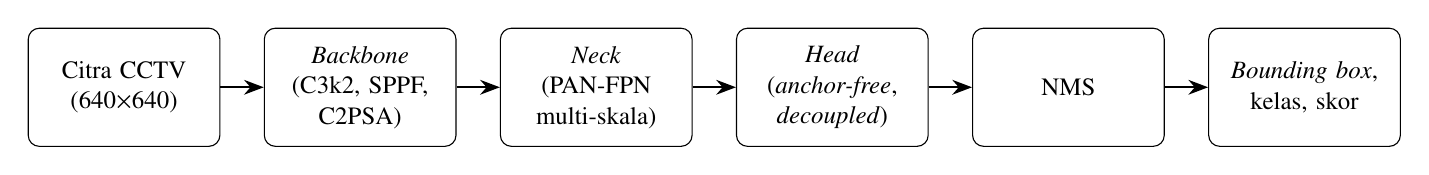
\begin{tikzpicture}[node distance=0.55cm,
        blok/.style={draw, rounded corners, minimum height=1.5cm, text width=2.2cm, align=center, font=\small},
        panah/.style={-{Stealth[length=2.5mm]}, thick}]
        \node[blok] (in) {Citra CCTV\\(640$\times$640)};
        \node[blok, right=of in] (bb) {\textit{Backbone}\\(C3k2, SPPF, C2PSA)};
        \node[blok, right=of bb] (nk) {\textit{Neck}\\(PAN-FPN multi-skala)};
        \node[blok, right=of nk] (hd) {\textit{Head}\\(\textit{anchor-free}, \textit{decoupled})};
        \node[blok, right=of hd] (nms) {NMS};
        \node[blok, right=of nms] (out) {\textit{Bounding box}, kelas, skor};
        \draw[panah] (in) -- (bb);
        \draw[panah] (bb) -- (nk);
        \draw[panah] (nk) -- (hd);
        \draw[panah] (hd) -- (nms);
        \draw[panah] (nms) -- (out);
    \end{tikzpicture}}
    \caption{Alur Arsitektur Detektor YOLO11n (Diolah dari \cite{ref36})}
    \label{fig:yolo}
\end{figure}

\subsection{Keterbatasan Memori GPU}
Memori GPU menjadi kendala utama dalam menjalankan VLM pada perangkat berkapasitas terbatas, yang jauh lebih terbatas dalam daya, termal, dan memori dibanding server \cite{ref14}. Penelitian ini menggunakan GPU konsumen NVIDIA GeForce RTX 5060 8 GB sebagai perangkat berkapasitas terbatas, dengan kapasitas VRAM yang dapat dipakai aplikasi sekitar 7,5 GiB karena sebagian dicadangkan oleh \textit{driver} (rincian pada Bab III). Kebutuhan memori GPU saat inferensi VLM tidak hanya ditentukan oleh bobot model, tetapi juga oleh \textit{key-value cache} (KV \textit{cache}) yang tumbuh seiring panjang urutan token, memori aktivasi sementara, serta \textit{overhead} sistem seperti konteks CUDA dan pustaka \textit{runtime}, sebagaimana diilustrasikan pada Gambar \ref{fig:vram}. Zheng dkk. \cite{ref32} melaporkan bahwa bobot BF16 model 7 miliar parameter menempati sekitar 16 GB sehingga tidak muat pada GPU 8 GB tanpa kuantisasi. Apabila kebutuhan memori melampaui kapasitas, inferensi berhenti karena kegagalan \textit{Out-of-Memory} (OOM), sehingga status OOM menjadi indikator apakah suatu konfigurasi model dan presisi dapat dijalankan secara stabil. Selain memori, latensi juga menjadi kendala karena pembangkitan teks secara autoregresif dilaporkan menyumbang lebih dari 85\% latensi ujung ke ujung VLM pada GPU berkapasitas terbatas \cite{ref24}.

\begin{figure}[htbp]
    \centering
    \resizebox{0.95\textwidth}{!}{%
    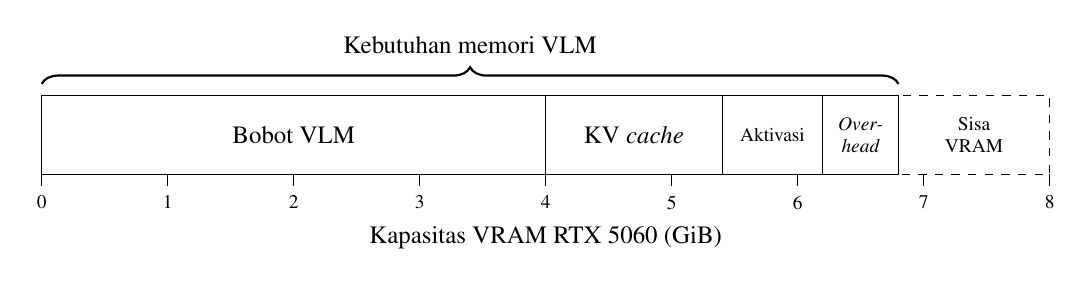
\begin{tikzpicture}[x=1.6cm, y=1cm]
        \draw (0,0) rectangle (4,1) node[midway, align=center, font=\small] {Bobot VLM};
        \draw (4,0) rectangle (5.4,1) node[midway, align=center, font=\small] {KV \textit{cache}};
        \draw (5.4,0) rectangle (6.2,1) node[midway, align=center, font=\scriptsize] {Aktivasi};
        \draw (6.2,0) rectangle (6.8,1) node[midway, align=center, font=\scriptsize] {\textit{Over-}\\\textit{head}};
        \draw[dashed] (6.8,0) rectangle (8,1) node[midway, align=center, font=\scriptsize] {Sisa\\VRAM};
        \foreach \x in {0,1,...,8} { \draw (\x,0) -- (\x,-0.15) node[below, font=\scriptsize] {\x}; }
        \node[font=\small] at (4,-0.8) {Kapasitas VRAM RTX 5060 (GiB)};
        \draw[decorate, decoration={brace, amplitude=6pt}, thick] (0,1.15) -- (6.8,1.15) node[midway, above=7pt, font=\small] {Kebutuhan memori VLM};
    \end{tikzpicture}}
    \caption{Ilustrasi Komponen Kebutuhan Memori VLM pada VRAM GPU}
    \label{fig:vram}
\end{figure}

\subsection{\textit{Vision-Language Model} (VLM)}
\textit{Vision-Language Model} (VLM) adalah model multimodal yang memproses masukan berupa citra dan teks secara bersamaan untuk menghasilkan keluaran berupa teks \cite{ref6}. Arsitektur VLM generatif umumnya terdiri atas enkoder visual berbasis \textit{Vision Transformer} (ViT) yang mengubah citra menjadi vektor fitur, proyektor antar-modalitas yang memetakannya ke ruang token teks, dan \textit{Large Language Model} (LLM) sebagai dekoder yang membangkitkan jawaban secara autoregresif token demi token, sebagaimana diilustrasikan pada Gambar \ref{fig:vlm} \cite{ref6}. Salah satu tugas utama VLM adalah \textit{Visual Question Answering} (VQA), yaitu menjawab pertanyaan berbahasa alami mengenai isi suatu citra, yang dapat dikerjakan secara \textit{zero-shot} tanpa pelatihan tambahan pada kelas atau domain tertentu \cite{ref6}. Kemampuan ini memungkinkan VLM menjawab pertanyaan yang tidak dapat ditangani detektor \textit{closed-set}, misalnya apakah seseorang berperan sebagai pegawai atau pelanggan, sehingga seluruh pengujian VLM dalam penelitian ini dirumuskan sebagai kueri VQA pada \textit{frame} tunggal \cite{ref22} dengan \textit{prompt} yang seragam untuk setiap model. Pada video pengawasan, VLM mampu menalar kejadian anomali tanpa pelatihan tambahan, tetapi menuntut sumber daya komputasi yang besar sehingga pada perangkat berkapasitas terbatas memerlukan kompresi \cite{ref14, ref22}.

\begin{figure}[htbp]
    \centering
    \resizebox{\textwidth}{!}{%
    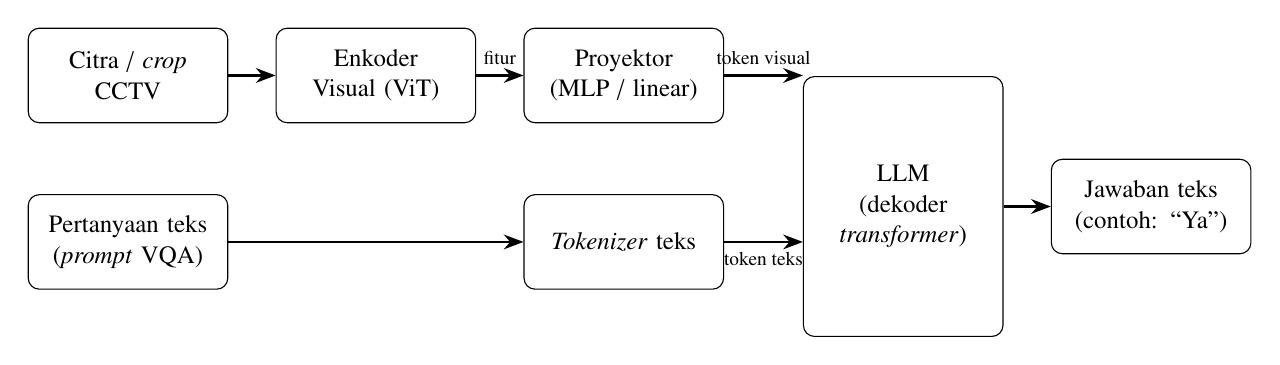
\begin{tikzpicture}[node distance=0.6cm,
        blok/.style={draw, rounded corners, minimum height=1.2cm, text width=2.3cm, align=center, font=\small},
        panah/.style={-{Stealth[length=2.5mm]}, thick}]
        \node[blok] (img) {Citra / \textit{crop} CCTV};
        \node[blok, right=of img] (enc) {Enkoder Visual (ViT)};
        \node[blok, right=of enc] (proj) {Proyektor (MLP / linear)};
        \node[blok, below=0.9cm of img] (txt) {Pertanyaan teks (\textit{prompt} VQA)};
        \node[blok, below=0.9cm of proj] (tok) {\textit{Tokenizer} teks};
        \node[blok, minimum height=3.3cm, right=1.0cm of proj.south east, anchor=north west, yshift=0.6cm] (llm) {LLM\\(dekoder \textit{transformer})};
        \node[blok, right=of llm] (ans) {Jawaban teks (contoh: ``Ya'')};
        \draw[panah] (img) -- (enc);
        \draw[panah] (enc) -- node[above, font=\scriptsize] {fitur} (proj);
        \draw[panah] (txt) -- (tok);
        \draw[panah] (proj.east) -- node[above, font=\scriptsize] {token visual} (proj.east -| llm.west);
        \draw[panah] (tok.east) -- node[below, font=\scriptsize] {token teks} (tok.east -| llm.west);
        \draw[panah] (llm) -- (ans);
    \end{tikzpicture}}
    \caption{Arsitektur Umum \textit{Vision-Language Model} Generatif (Diolah dari \cite{ref6})}
    \label{fig:vlm}
\end{figure}

Keempat VLM yang diuji merupakan variabel bebas pertama, mewakili keluarga model terbuka yang berbeda dalam enkoder visual, LLM, dan ukuran sekitar 2--4 miliar parameter, dengan estimasi memori bobot pada Tabel \ref{tab:model} yang dihitung dari jumlah parameter dan jumlah \textit{byte} per parameter (Subbab \ref{sub:kuantisasi}) sehingga kebutuhan aktual lebih besar setelah ditambah KV \textit{cache}, aktivasi, dan \textit{overhead}. PaliGemma 2 menggabungkan enkoder SigLIP dengan LLM Gemma 2, dan varian \textit{mix} dipakai agar model dapat langsung menjawab kueri VQA tanpa \textit{fine-tuning}\footnote{Spesifikasi resmi model: \url{https://huggingface.co/google/paligemma2-3b-mix-448}}, sedangkan Qwen2.5-VL varian \textit{Instruct} memproses citra pada resolusi aslinya secara dinamis sehingga jumlah token visual dan KV \textit{cache} bergantung pada ukuran masukan\footnote{Spesifikasi resmi model: \url{https://huggingface.co/Qwen/Qwen2.5-VL-3B-Instruct}}. InternVL2.5 4B menggabungkan enkoder InternViT-300M dengan LLM Qwen2.5-3B melalui proyektor \textit{Multi-Layer Perceptron} (MLP) \cite{ref29}, sedangkan Moondream2 adalah VLM ringkas berukuran sekitar 1,9 miliar parameter yang menggabungkan SigLIP dengan Phi-1.5\footnote{Spesifikasi resmi model: \url{https://huggingface.co/vikhyatk/moondream2}} \cite{ref14} dan telah dipakai untuk mendeskripsikan insiden jalan raya \cite{ref31}. Pengukuran awal pada RTX 5060 mencatat bobot BF16 InternVL2.5 4B sebesar 7,02 GiB (sekitar 7,5 GB) dan bobot BF16 Qwen2.5-VL-3B diperkirakan sekitar 7,5 GB, sehingga keduanya hampir menghabiskan VRAM yang dapat dipakai aplikasi dan paling bergantung pada kuantisasi, sedangkan Moondream2 (sekitar 3,8 GB pada BF16) diperkirakan dapat berjalan tanpa kuantisasi. Perbedaan ukuran dan rancangan keempat model diperkirakan memengaruhi jejak memori, latensi, dan tingkat halusinasi, dengan Moondream2 sebagai model terkecil yang menjadi batas bawah untuk menguji apakah pengurangan parameter berdampak lebih besar terhadap halusinasi dibanding kuantisasi.

\begin{table}[htbp]
    \centering
    \caption{Spesifikasi dan Estimasi Memori Bobot VLM yang Diuji}
    \label{tab:model}
    \renewcommand{\arraystretch}{1.3}
    \small
    \begin{tabular}{|p{2.6cm}|p{2.4cm}|p{2.2cm}|c|c|c|c|}
    \hline
    \multirow{2}{*}{\textbf{Model}} & \multirow{2}{*}{\textbf{Enkoder Visual}} & \multirow{2}{*}{\textbf{LLM}} & \multirow{2}{*}{\textbf{Param.}} & \multicolumn{3}{c|}{\textbf{Estimasi Memori Bobot (GB)}} \\
    \cline{5-7}
    & & & & \textbf{BF16} & \textbf{INT8} & \textbf{NF4} \\
    \hline
    PaliGemma 2 3B & SigLIP-So400m & Gemma 2 2B & $\pm$3,0B & 6,0 & 3,0 & 1,5 \\
    \hline
    Qwen2.5-VL-3B & ViT \textit{window attention} & Qwen2.5 3B & $\pm$3,8B & 7,5 & 3,8 & 1,9 \\
    \hline
    InternVL2.5 4B \cite{ref29} & InternViT-300M & Qwen2.5 3B & $\pm$3,7B & 7,4 & 3,7 & 1,9 \\
    \hline
    Moondream2 & SigLIP & Phi-1.5 & $\pm$1,9B & 3,8 & 1,9 & 1,0 \\
    \hline
    \end{tabular}

    % REVISI R7: catatan estimasi ditambahkan (enkoder visual dan proyektor tetap BF16)
    \vspace{1ex}
    {\footnotesize Catatan: estimasi INT8 dan NF4 mengasumsikan seluruh parameter dikuantisasi. Karena enkoder visual dan proyektor dipertahankan pada BF16 (Subbab \ref{sec:persiapan}), kebutuhan aktualnya lebih besar, terutama pada NF4.\par}
\end{table}

\subsection{Presisi dan Kuantisasi Bobot: BF16, INT8, dan NF4}
\label{sub:kuantisasi}
Presisi bobot menyatakan jumlah bit dan format bilangan yang digunakan untuk menyimpan setiap bobot model, sehingga menentukan besar memori yang ditempati dan seberapa halus nilai bobot direpresentasikan. Penelitian ini menguji tiga tingkat presisi sebagai variabel bebas kedua. BF16 (\textit{Brain Floating Point} 16-bit) adalah format bilangan titik mengambang 16-bit dengan 1 bit tanda, 8 bit eksponen, dan 7 bit mantisa, yang umum digunakan dalam pelatihan jaringan saraf dalam dan di sini dipakai sebagai presisi asli tanpa kuantisasi. INT8 adalah representasi bobot sebagai bilangan bulat 8-bit. \textit{NormalFloat} 4-bit (NF4) adalah tipe data 4-bit yang dirancang optimal secara teori informasi untuk bobot yang berdistribusi normal, dengan 16 nilai kuantil distribusi normal baku sebagai nilai representasinya \cite{ref35}. Dampak langsung presisi terhadap memori dapat diestimasi dari jumlah parameter dikalikan jumlah \textit{byte} per parameter, yaitu 2 \textit{byte} untuk BF16, 1 \textit{byte} untuk INT8, dan sekitar 0,5 \textit{byte} untuk NF4. Estimasi ini belum memperhitungkan faktor skala, konstanta normalisasi, dan lapisan yang tetap disimpan dalam presisi tinggi, sehingga nilai aktual sedikit lebih besar.

Kuantisasi adalah proses menurunkan presisi bobot, yaitu merepresentasikan bobot berpresisi tinggi menggunakan tipe data berpresisi rendah sehingga kebutuhan memori berkurang. Teknik ini dibutuhkan pada perangkat berkapasitas terbatas, yang memiliki keterbatasan dalam daya pemrosesan, memori, dan energi sehingga memerlukan kompresi model seperti kuantisasi, pemangkasan, dan distilasi \cite{ref14}. Kuantisasi pasca-pelatihan (\textit{post-training quantization}) dilakukan setelah model selesai dilatih sehingga tidak memerlukan pelatihan ulang. Pada prinsipnya, setiap bobot dipetakan ke salah satu dari sejumlah nilai diskret yang terbatas menggunakan faktor skala, dan selisih antara bobot asli dan bobot hasil dekuantisasi disebut galat kuantisasi, yang menjadi sumber penurunan akurasi model. Presisi INT8 dihasilkan oleh metode seperti LLM.int8(), yang memakai faktor skala per vektor dan menangani sebagian kecil dimensi fitur berskala besar (\textit{outlier}) secara terpisah dalam presisi 16-bit, serta dilaporkan mengurangi memori inferensi sekitar setengahnya tanpa penurunan kinerja pada model berukuran besar \cite{ref34}. Presisi NF4 dihasilkan oleh metode QLoRA, yang membagi bobot ke dalam blok, menormalisasi setiap blok dengan nilai mutlak maksimumnya ke rentang $-1$ sampai $1$, lalu memetakan setiap nilai ke nilai NF4 terdekat, sedangkan konstanta normalisasi setiap blok dikuantisasi sekali lagi (\textit{double quantization}) untuk menekan memori tambahan \cite{ref35}. Penghematan memori belum tentu mempercepat inferensi, dan penurunan presisi berpotensi melemahkan kemampuan model dalam memverifikasi isi citra sehingga meningkatkan kecenderungan halusinasi. Hubungan antara penghematan memori, latensi, dan perubahan halusinasi inilah yang diukur dalam penelitian ini.

\subsection{Halusinasi Objek dan Evaluasi POPE}
Halusinasi objek adalah kondisi ketika VLM menyatakan keberadaan objek yang tidak terdapat pada citra, dan paling sering terjadi pada objek yang sering muncul dalam data latih atau sering hadir bersama objek lain \cite{ref9}. Pada CCTV, halusinasi berarti alarm palsu, misalnya menyatakan adanya aktivitas transaksi yang tidak pernah terjadi, sehingga tingkat halusinasi menjadi variabel terikat yang krusial dalam menilai kelayakan VLM, terlebih karena penurunan presisi akibat kuantisasi berpotensi meningkatkannya. \textit{Polling-based Object Probing Evaluation} (POPE) menilai halusinasi melalui kueri biner berbentuk ``Apakah terdapat \textless objek\textgreater{} pada citra?'', dengan kueri positif dari objek yang ada pada anotasi dan kueri negatif dari objek yang tidak ada, yang dipilih secara acak (\textit{random}), paling sering muncul (\textit{popular}), atau sering muncul bersamaan dengan objek pada citra (\textit{adversarial}) \cite{ref9}. Format biner ini membuat evaluasi lebih stabil dibanding metode berbasis \textit{caption} yang dipengaruhi gaya keluaran model, dan jawaban model dikelompokkan ke dalam matriks konfusi seperti pada Gambar \ref{fig:konfusi} \cite{ref9}.

\begin{figure}[htbp]
    \centering
    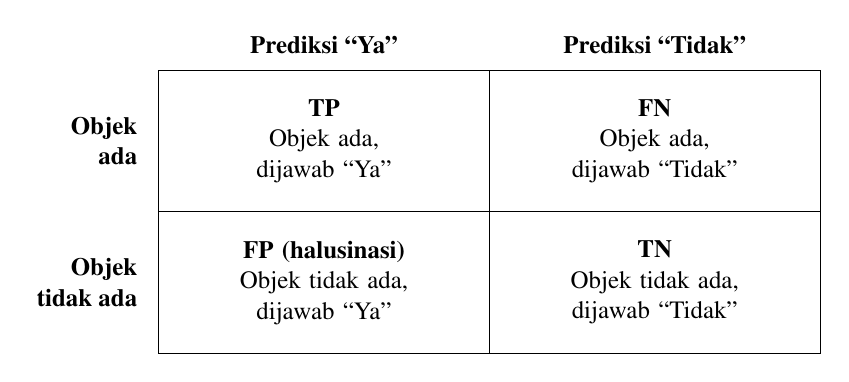
\begin{tikzpicture}[sel/.style={draw, minimum width=4.2cm, minimum height=1.8cm, text width=3.8cm, align=center, font=\small}]
        \node[sel] (tp) at (0,0) {\textbf{TP}\\Objek ada,\\dijawab ``Ya''};
        \node[sel] (fn) at (4.2,0) {\textbf{FN}\\Objek ada,\\dijawab ``Tidak''};
        \node[sel] (fp) at (0,-1.8) {\textbf{FP (halusinasi)}\\Objek tidak ada,\\dijawab ``Ya''};
        \node[sel] (tn) at (4.2,-1.8) {\textbf{TN}\\Objek tidak ada,\\dijawab ``Tidak''};
        \node[font=\small\bfseries, above=2pt of tp] {Prediksi ``Ya''};
        \node[font=\small\bfseries, above=2pt of fn] {Prediksi ``Tidak''};
        \node[font=\small\bfseries, left=4pt of tp, align=right] {Objek\\ada};
        \node[font=\small\bfseries, left=4pt of fp, align=right] {Objek\\tidak ada};
    \end{tikzpicture}
    \caption{Matriks Konfusi pada Evaluasi Halusinasi Berbasis POPE (Diolah dari \cite{ref9})}
    \label{fig:konfusi}
\end{figure}

Berdasarkan matriks konfusi tersebut, POPE melaporkan metrik \textit{accuracy}, \textit{precision}, \textit{recall}, F1-\textit{score}, dan rasio jawaban ``Ya'' \cite{ref9}, sedangkan penelitian ini mendefinisikan \textit{Object Hallucination Rate} (OHR) sebagai proporsi kueri negatif yang dijawab ``Ya'' oleh model, sebagaimana dirumuskan pada Persamaan \eqref{eq:ohr}. Nilai OHR yang tinggi menandakan model mudah berhalusinasi, sedangkan rasio jawaban ``Ya'' jauh di atas 50\% menunjukkan kecenderungan selalu mengiyakan. Perubahan OHR akibat kuantisasi dihitung sebagai selisih antara OHR model terkuantisasi dan OHR model berpresisi asli (BF16), sebagaimana Persamaan \eqref{eq:dohr}.
\begin{equation}
OHR = \frac{FP}{FP + TN} \times 100\%
\label{eq:ohr}
\end{equation}
\begin{equation}
\Delta OHR = OHR_{kuantisasi} - OHR_{asli}
\label{eq:dohr}
\end{equation}
dengan $FP$ jumlah kueri negatif yang dijawab ``Ya'' dan $TN$ yang dijawab ``Tidak''.

\subsection{Metrik Evaluasi Klasifikasi dan Kinerja Inferensi}
Akurasi klasifikasi peran dan jawaban POPE dievaluasi menggunakan matriks konfusi, dengan kelas positif berupa pegawai atau objek ada, melalui \textit{accuracy}, \textit{precision}, \textit{recall}, dan F1-\textit{score} sebagaimana Persamaan \eqref{eq:acc} hingga \eqref{eq:f1} \cite{ref2}.
\begin{equation}
Accuracy = \frac{TP + TN}{TP + TN + FP + FN}
\label{eq:acc}
\end{equation}
\begin{equation}
Precision = \frac{TP}{TP + FP}, \qquad Recall = \frac{TP}{TP + FN}
\label{eq:pr}
\end{equation}
\begin{equation}
F1 = 2 \times \frac{Precision \times Recall}{Precision + Recall}
\label{eq:f1}
\end{equation}
Kinerja inferensi dinilai dari penggunaan memori GPU, status OOM, dan latensi, yaitu waktu sejak kueri dan citra diterima hingga jawaban selesai dibangkitkan. Pembangkitan teks autoregresif menyumbang lebih dari 85\% latensi ujung ke ujung \cite{ref24}. Latensi dilaporkan sebagai rata-rata dari sejumlah pengulangan kueri sebagaimana Persamaan \eqref{eq:lat}.
\begin{equation}
\bar{t} = \frac{1}{N} \sum_{i=1}^{N} \left(t_{selesai,i} - t_{mulai,i}\right)
\label{eq:lat}
\end{equation}
dengan $N$ jumlah kueri serta $t_{mulai,i}$ dan $t_{selesai,i}$ waktu mulai dan selesai kueri ke-$i$.

\cleardoublepage
\chapter{METODOLOGI PENELITIAN}

\section{Jenis dan Desain Penelitian}
Penelitian ini merupakan penelitian kuantitatif dengan pendekatan eksperimental komparatif. Pendekatan eksperimental dipilih karena penelitian ini secara sengaja memvariasikan arsitektur VLM dan tingkat presisi bobot, lalu mengukur dampaknya secara numerik. Desain utama berbentuk faktorial $4 \times 3$, yaitu empat arsitektur VLM yang masing-masing diuji pada tiga tingkat presisi sehingga menghasilkan dua belas konfigurasi. Seluruh konfigurasi diuji menggunakan data, \textit{prompt}, dan perangkat keras yang sama agar perbedaan hasil hanya disebabkan oleh variabel yang diteliti. Komponen deteksi dan pelacakan (YOLO11n dan ByteTrack) dibuat tetap sehingga perbedaan hasil dapat dikaitkan dengan jenis VLM dan presisinya. Hasil seluruh eksperimen dianalisis secara deskriptif dan komparatif untuk menjawab ketiga rumusan masalah.

\section{Variabel Penelitian}
Variabel penelitian ditetapkan berdasarkan rumusan masalah dan landasan teori pada Bab II. Variabel bebas adalah faktor yang sengaja divariasikan, variabel terikat adalah hasil yang diukur, dan variabel kontrol adalah faktor yang dijaga tetap agar perbandingan bersifat adil. Setiap variabel terikat diukur menggunakan metrik yang telah dijelaskan pada Bab II sehingga hasilnya dapat dibandingkan secara konsisten. Variabel kontrol menjadi bagian penting karena VLM sangat sensitif terhadap perbedaan \textit{prompt}, resolusi masukan, dan pengaturan pembangkitan teks. Rincian seluruh variabel beserta satuan dan keterkaitannya dengan rumusan masalah disajikan pada Tabel \ref{tab:variabel}.

{\renewcommand{\arraystretch}{1.3}
\begin{longtable}{|c|>{\raggedright\arraybackslash}p{5.6cm}|>{\raggedright\arraybackslash}p{5.2cm}|c|}
    \caption{Variabel Penelitian}
    \label{tab:variabel} \\
    \hline
    \textbf{No} & \textbf{Variabel} & \textbf{Satuan / Nilai} & \textbf{RM} \\
    \hline
    \endfirsthead
    \caption[]{Variabel Penelitian \textit{(Lanjutan)}} \\
    \hline
    \textbf{No} & \textbf{Variabel} & \textbf{Satuan / Nilai} & \textbf{RM} \\
    \hline
    \endhead
    \multicolumn{4}{|l|}{\textbf{Variabel Bebas}} \\
    \hline
    1 & Arsitektur VLM & PaliGemma 2, Qwen2.5-VL, InternVL2.5, Moondream2 & 1, 2, 3 \\
    \hline
    2 & Tingkat presisi bobot & BF16 (asli), INT8, NF4 & 1, 2, 3 \\
    \hline
    \multicolumn{4}{|l|}{\textbf{Variabel Terikat}} \\
    \hline
    1 & Jejak memori puncak & GiB & 1 \\
    \hline
    2 & Status OOM & Ya / Tidak & 1 \\
    \hline
    3 & Latensi rata-rata VLM ($\bar{t}$) & milidetik per kueri & 1 \\
    \hline
    4 & OHR dan $\Delta OHR$, ditambah metrik POPE & \% & 2 \\
    \hline
    5 & \textit{Accuracy}, \textit{precision}, \textit{recall}, F1 klasifikasi peran & \% & 3 \\
    \hline
    \multicolumn{4}{|l|}{\textbf{Variabel Kontrol}} \\
    \hline
    1 & Perangkat keras uji & NVIDIA RTX 5060 8 GB & -- \\
    \hline
    2 & Detektor dan pelacak & YOLO11n + ByteTrack \textit{pretrained}, tanpa \textit{fine-tuning} & -- \\
    \hline
    3 & Dataset uji & \textit{Frame} yang sama untuk semua konfigurasi & -- \\
    \hline
    4 & \textit{Prompt} kueri & Templat yang sama untuk semua model & -- \\
    \hline
    5 & Resolusi masukan VLM & Dibatasi seragam & -- \\
    \hline
    6 & Pengaturan pembangkitan & \textit{Greedy}, \textit{batch} 1, token keluaran dibatasi & -- \\
    \hline
\end{longtable}
}

\section{Bahan dan Peralatan Penelitian}
% REVISI R2: kalimat GPU pembanding diganti (seluruh pengukuran pada satu GPU)
Peralatan penelitian dipilih untuk merepresentasikan perangkat berkapasitas terbatas kelas konsumen. Komponen utama adalah GPU NVIDIA GeForce RTX 5060 dengan VRAM 8 GB yang digunakan untuk seluruh pengukuran memori, latensi, halusinasi objek, dan klasifikasi peran. Seluruh pengukuran dilakukan pada GPU yang sama sehingga tidak ada perbandingan lintas-GPU. Perangkat lunak dipilih berdasarkan kompatibilitasnya dengan arsitektur GPU yang digunakan dan ketersediaan dukungan kuantisasi untuk keempat model. Rincian perangkat keras dan perangkat lunak disajikan pada Tabel \ref{tab:hardware} dan Tabel \ref{tab:software}.

\begin{table}[H]
    \centering
    \caption{Spesifikasi Perangkat Keras}
    \label{tab:hardware}
    \renewcommand{\arraystretch}{1.3}
    \begin{tabular}{|c|p{4cm}|p{8cm}|}
    \hline
    \textbf{No} & \textbf{Komponen} & \textbf{Spesifikasi dan Fungsi} \\
    \hline
    % REVISI R1: baris "GPU pembanding" dihapus, nomor baris digeser
    1 & GPU uji & NVIDIA GeForce RTX 5060 8 GB VRAM, untuk seluruh pengukuran (memori, latensi, halusinasi objek, dan klasifikasi peran) \\
    \hline
    2 & CPU & Intel Core i5 / AMD Ryzen 5 atau setara \\
    \hline
    3 & RAM & 16 GB atau lebih \\
    \hline
    4 & Penyimpanan & SSD NVMe 512 GB \\
    \hline
    5 & Sumber data video & Rekaman CCTV tempat usaha (1080p) \\
    \hline
    \end{tabular}
\end{table}

\begin{table}[H]
    \centering
    \caption{Spesifikasi Perangkat Lunak}
    \label{tab:software}
    \renewcommand{\arraystretch}{1.3}
    \begin{tabular}{|c|p{4.5cm}|p{7.5cm}|}
    \hline
    \textbf{No} & \textbf{Perangkat Lunak} & \textbf{Fungsi} \\
    \hline
    % REVISI R6: versi Ubuntu dan Transformers disesuaikan dengan mesin uji
    1 & Ubuntu 22.04 atau 24.04 LTS & Sistem operasi (mesin uji memakai 24.04) \\
    \hline
    2 & Python 3.10 atau lebih baru & Bahasa pemrograman \\
    \hline
    3 & NVIDIA CUDA 12.8 atau lebih baru & Lingkungan komputasi GPU (syarat minimum arsitektur Blackwell pada RTX 5060) \\
    \hline
    4 & PyTorch 2.7 atau lebih baru & \textit{Framework deep learning} \\
    \hline
    5 & Ultralytics & Deteksi YOLO11n dan pelacakan ByteTrack \\
    \hline
    6 & Hugging Face \textit{Transformers} seri 4.x & Pemuatan dan inferensi VLM. Versi 5.20.1 gagal memuat InternVL2.5 4B (galat \texttt{all\_tied\_weights\_keys}), sedangkan versi 4.57.6 berhasil \\
    \hline
    7 & \textit{bitsandbytes} & Kuantisasi INT8 (LLM.int8()) dan NF4 (QLoRA) \\
    \hline
    8 & OpenCV & Pengolahan citra dan pemotongan (\textit{crop}) orang \\
    \hline
    9 & NVML (\texttt{pynvml}) & Pemantauan pemakaian VRAM \\
    \hline
    10 & CVAT / Label Studio & Anotasi objek dan peran \\
    \hline
    \end{tabular}
\end{table}

\section{Diagram Alir Penelitian}
Tahapan penelitian disusun secara berurutan mulai dari studi literatur hingga penarikan kesimpulan, sebagaimana ditunjukkan pada Gambar \ref{fig:flowchart}. Setelah data dan komponen deteksi YOLO11n disiapkan, setiap konfigurasi model dan presisi diuji satu per satu pada GPU uji. Apabila suatu konfigurasi mengalami OOM, kondisi tersebut dicatat sebagai hasil bahwa konfigurasi tidak stabil, lalu pengujian berlanjut ke konfigurasi berikutnya. Konfigurasi yang berhasil dimuat dilanjutkan ke pengujian memori dan latensi, halusinasi, serta klasifikasi peran. Setelah seluruh konfigurasi selesai diuji, hasilnya dianalisis secara komparatif untuk menarik kesimpulan.

\begin{figure}[htbp]
    \centering
    \resizebox{!}{0.62\textheight}{%
    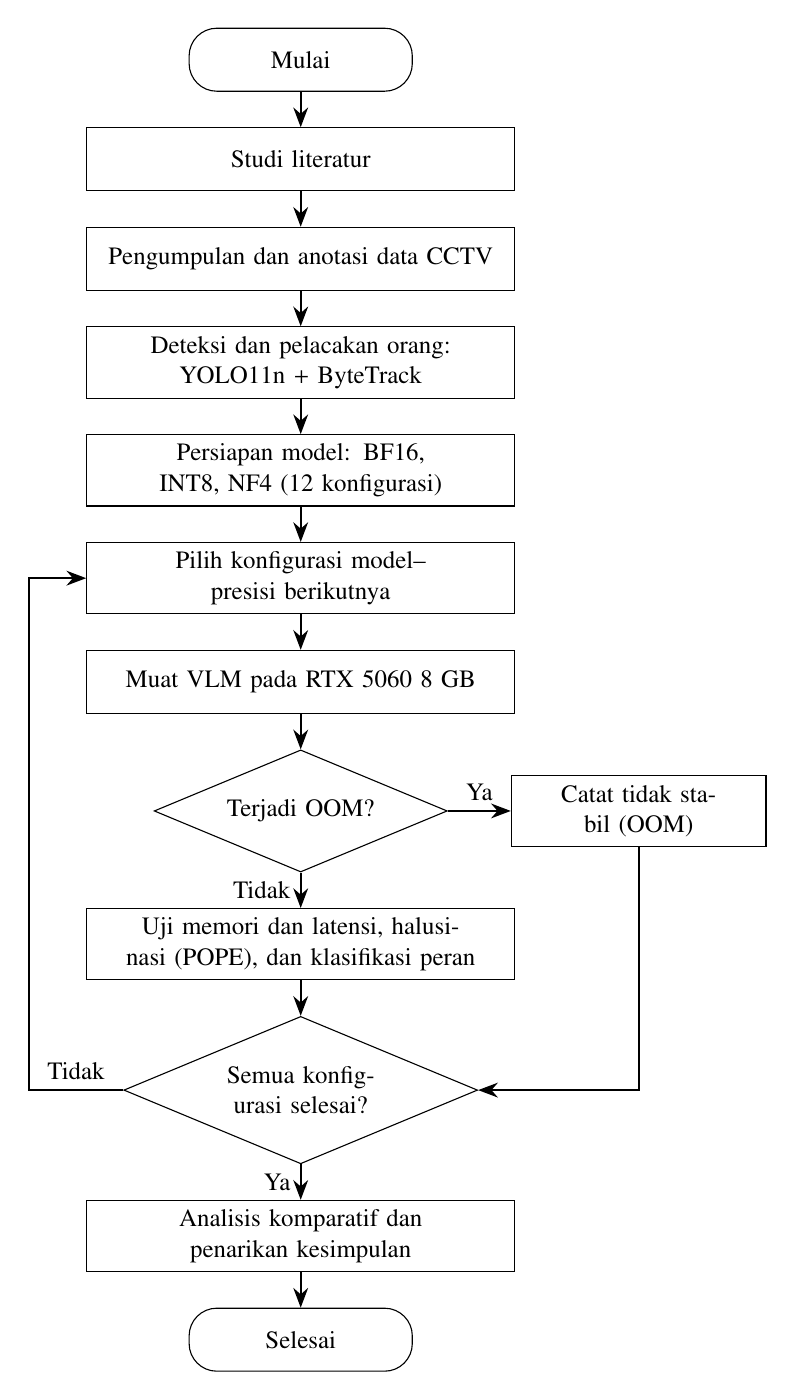
\begin{tikzpicture}[node distance=0.45cm,
        term/.style={draw, rounded corners=10pt, minimum height=0.8cm, text width=2.6cm, align=center, font=\small},
        proses/.style={draw, minimum height=0.8cm, text width=5.2cm, align=center, font=\small},
        cek/.style={draw, diamond, aspect=2.4, inner sep=1pt, text width=2.8cm, align=center, font=\small},
        panah/.style={-{Stealth[length=2.5mm]}, thick}]
        \node[term] (mulai) {Mulai};
        \node[proses, below=of mulai] (lit) {Studi literatur};
        \node[proses, below=of lit] (data) {Pengumpulan dan anotasi data CCTV};
        \node[proses, below=of data] (yolo) {Deteksi dan pelacakan orang: YOLO11n + ByteTrack};
        \node[proses, below=of yolo] (kuant) {Persiapan model: BF16, INT8, NF4 (12 konfigurasi)};
        \node[proses, below=of kuant] (pilih) {Pilih konfigurasi model--presisi berikutnya};
        \node[proses, below=of pilih] (muat) {Muat VLM pada RTX 5060 8 GB};
        \node[cek, below=of muat] (oom) {Terjadi OOM?};
        \node[proses, right=0.8cm of oom, text width=3.0cm] (catat) {Catat tidak stabil (OOM)};
        \node[proses, below=of oom] (uji) {Uji memori dan latensi, halusinasi (POPE), dan klasifikasi peran};
        \node[cek, below=of uji] (semua) {Semua konfigurasi selesai?};
        \node[proses, below=of semua] (analisis) {Analisis komparatif dan penarikan kesimpulan};
        \node[term, below=of analisis] (selesai) {Selesai};
        \draw[panah] (mulai) -- (lit);
        \draw[panah] (lit) -- (data);
        \draw[panah] (data) -- (yolo);
        \draw[panah] (yolo) -- (kuant);
        \draw[panah] (kuant) -- (pilih);
        \draw[panah] (pilih) -- (muat);
        \draw[panah] (muat) -- (oom);
        \draw[panah] (oom) -- node[above, font=\small] {Ya} (catat);
        \draw[panah] (oom) -- node[left, font=\small] {Tidak} (uji);
        \draw[panah] (uji) -- (semua);
        \draw[panah] (catat.south) |- (semua.east);
        \draw[panah] (semua.west) -- node[above, font=\small] {Tidak} ++(-1.2,0) |- (pilih.west);
        \draw[panah] (semua) -- node[left, font=\small] {Ya} (analisis);
        \draw[panah] (analisis) -- (selesai);
    \end{tikzpicture}}
    \caption{Diagram Alir Penelitian}
    \label{fig:flowchart}
\end{figure}

\section{Rancangan Sistem}
Sistem yang diuji terdiri atas dua lapisan, yaitu lapisan deteksi dan pelacakan serta lapisan penalaran semantik, sebagaimana ditunjukkan pada Gambar \ref{fig:arsitektur}. Lapisan deteksi menjalankan YOLO11n dan ByteTrack pada \textit{frame} uji untuk menghasilkan kotak deteksi beserta identitas lintasan setiap orang, yang kemudian dipotong menjadi \textit{crop} sebagai masukan VLM. Lapisan penalaran semantik berupa VLM yang menerima \textit{crop} atau \textit{frame} beserta kueri VQA dan menjawab dalam bentuk teks. Komponen deteksi dan pelacakan dibuat tetap, sedangkan VLM divariasikan dalam arsitektur dan tingkat presisinya sehingga perbedaan hasil dapat dikaitkan dengan kedua faktor tersebut.

\begin{figure}[htbp]
    \centering
    \resizebox{\textwidth}{!}{%
    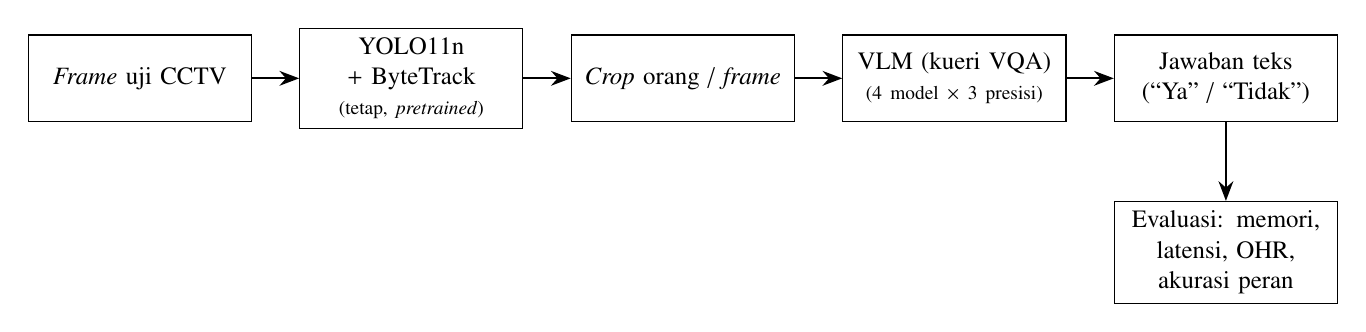
\begin{tikzpicture}[node distance=0.6cm,
        blok/.style={draw, minimum height=1.1cm, text width=2.6cm, align=center, font=\small},
        panah/.style={-{Stealth[length=2.5mm]}, thick}]
        \node[blok] (cam) {\textit{Frame} uji CCTV};
        \node[blok, right=of cam] (det) {YOLO11n + ByteTrack\\{\scriptsize (tetap, \textit{pretrained})}};
        \node[blok, right=of det] (crop) {\textit{Crop} orang / \textit{frame}};
        \node[blok, right=of crop] (vlm) {VLM (kueri VQA)\\{\scriptsize (4 model $\times$ 3 presisi)}};
        \node[blok, right=of vlm] (jwb) {Jawaban teks (``Ya'' / ``Tidak'')};
        \node[blok, below=1.0cm of jwb] (evl) {Evaluasi: memori, latensi, OHR, akurasi peran};
        \draw[panah] (cam) -- (det);
        \draw[panah] (det) -- (crop);
        \draw[panah] (crop) -- (vlm);
        \draw[panah] (vlm) -- (jwb);
        \draw[panah] (jwb) -- (evl);
    \end{tikzpicture}}
    \caption{Rancangan Sistem yang Diuji}
    \label{fig:arsitektur}
\end{figure}

\section{Pengumpulan dan Anotasi Data}
Penelitian ini tidak melatih model sehingga data yang dikumpulkan berfungsi sebagai data uji. Data utama berupa 200--300 \textit{frame} yang diekstraksi dari rekaman CCTV tempat usaha dengan variasi kepadatan orang, oklusi, dan kondisi pencahayaan. \textit{Frame} yang sama digunakan untuk setiap konfigurasi sehingga perbandingan antarkonfigurasi bersifat adil.

Anotasi dilakukan secara manual dan mencakup dua jenis label yang disesuaikan dengan kebutuhan setiap skenario pengujian. Pertama, anotasi keberadaan objek berupa daftar kategori objek yang terdapat pada setiap \textit{frame}, seperti orang, tas, keranjang belanja, ponsel, dan mesin kasir, yang menjadi dasar penyusunan kueri POPE. Kedua, anotasi peran berupa label pegawai atau pelanggan untuk setiap orang yang terdeteksi, yang menjadi \textit{ground truth} skenario klasifikasi peran.

Kueri POPE disusun dari anotasi keberadaan objek mengikuti protokol yang dijelaskan pada Bab II. Setiap \textit{frame} menghasilkan tiga kueri positif dari objek yang ada dan tiga kueri negatif dari objek yang tidak ada untuk masing-masing strategi \textit{random}, \textit{popular}, dan \textit{adversarial}. Dengan 250 \textit{frame}, rancangan ini menghasilkan sekitar 4.500 kueri biner untuk setiap konfigurasi model, dan jumlah tersebut dapat disesuaikan dengan ketersediaan objek pada data. Seluruh kueri menggunakan templat yang sama, yaitu ``Apakah terdapat \textless objek\textgreater{} pada gambar ini? Jawab hanya dengan Ya atau Tidak.'' dalam bahasa yang sama untuk semua model. Keseragaman templat ini menjadi variabel kontrol agar perbedaan OHR tidak disebabkan oleh perbedaan \textit{prompt}.

\section{Persiapan dan Kuantisasi Model}
Keempat VLM diunduh dalam bentuk \textit{pretrained} dari repositori resminya dan digunakan tanpa \textit{fine-tuning}. Untuk PaliGemma 2 digunakan varian \textit{mix} yang telah dilatih pada campuran tugas, sedangkan untuk Qwen2.5-VL digunakan varian \textit{Instruct}, agar seluruh model dapat langsung menjawab kueri VQA. Setiap model disiapkan dalam tiga tingkat presisi, yaitu BF16 sebagai presisi asli tanpa kuantisasi, INT8 menggunakan LLM.int8(), dan NF4 menggunakan QLoRA, yang keduanya tersedia melalui pustaka \textit{bitsandbytes}. Kuantisasi diterapkan pada LLM yang merupakan komponen terbesar, sedangkan enkoder visual dan proyektor dipertahankan pada presisi asli untuk menjaga kualitas fitur visual. Kuantisasi bersifat pasca-pelatihan sehingga tidak memerlukan data kalibrasi maupun pelatihan ulang. Kedua belas konfigurasi yang dihasilkan disajikan pada Tabel \ref{tab:konfigurasi}.

\begin{table}[htbp]
    \centering
    \caption{Matriks Konfigurasi Eksperimen}
    \label{tab:konfigurasi}
    \renewcommand{\arraystretch}{1.3}
    \begin{tabular}{|p{3.6cm}|c|c|c|}
    \hline
    \textbf{Model} & \textbf{BF16 (asli)} & \textbf{INT8} & \textbf{NF4} \\
    \hline
    PaliGemma 2 3B (\textit{mix}) & K1 & K2 & K3 \\
    \hline
    Qwen2.5-VL-3B-Instruct & K4 & K5 & K6 \\
    \hline
    InternVL2.5 4B & K7 & K8 & K9 \\
    \hline
    Moondream2 & K10 & K11 & K12 \\
    \hline
    \end{tabular}
\end{table}

\section{Skenario Pengujian}
Pengujian dilakukan melalui tiga skenario yang masing-masing menjawab satu rumusan masalah, dengan pengaturan seragam berupa \textit{greedy decoding}, \textit{batch} satu, jumlah token keluaran terbatas, dan resolusi citra seragam. Setiap konfigurasi menjalani kueri pemanasan (\textit{warm-up}) sebelum pengukuran, dan jejak memori puncak diukur melalui NVML (\texttt{pynvml}) dikurangi \textit{baseline} kondisi \textit{idle}. Pengukuran dijalankan melalui sesi SSH tanpa lingkungan desktop agar VRAM tidak terpakai, dengan VRAM yang dapat dipakai aplikasi sekitar 7,5 GiB dari 8 GB nominal karena $\pm$461 MiB dicadangkan \textit{driver}. Memori dilaporkan dalam GiB (1 GiB = $2^{30}$ byte), sedangkan estimasi bobot pada Tabel \ref{tab:model} dalam GB (1 GB = $10^{9}$ byte). Kestabilan dan keandalan konfigurasi menjadi dasar keputusan setiap skenario, yaitu apakah konfigurasi dapat diuji lebih lanjut dan mana yang paling stabil, dengan batas keputusan pada Tabel \ref{tab:standar}.
%
% OPSIONAL (usulan, tanyakan pembimbing dulu; hapus tanda % pada baris berikut bila disetujui):
% Frekuensi \textit{clock} GPU dikunci pada 2092 MHz agar seluruh konfigurasi diukur pada kondisi termal yang sama.

{\small
\renewcommand{\arraystretch}{1.3}
\begin{longtable}{|c|>{\raggedright\arraybackslash}p{1.9cm}|>{\raggedright\arraybackslash}p{3.0cm}|>{\raggedright\arraybackslash}p{3.9cm}|>{\raggedright\arraybackslash}p{4.2cm}|}
    \caption{Standar Keputusan Kestabilan dan Keandalan Konfigurasi pada Setiap Pengujian}
    \label{tab:standar} \\
    \hline
    \textbf{No} & \textbf{Pengujian} & \textbf{Indikator} & \textbf{Batas} & \textbf{Keputusan} \\
    \hline
    \endfirsthead
    \caption[]{Standar Keputusan Kestabilan dan Keandalan Konfigurasi pada Setiap Pengujian \textit{(Lanjutan)}} \\
    \hline
    \textbf{No} & \textbf{Pengujian} & \textbf{Indikator} & \textbf{Batas} & \textbf{Keputusan} \\
    \hline
    \endhead
    1 & \multirow{3}{*}{Skenario 1} & Kejadian OOM & Maksimum 0 kejadian pada seluruh kueri. & Jika terlampaui, konfigurasi tidak stabil dan tidak diuji pada Skenario 2 dan 3. \\*
    \cline{1-1}\cline{3-5}
    2 & & Jejak memori puncak & Maksimum 90\% VRAM yang dapat dipakai aplikasi ($\pm$6,75 GiB dari $\pm$7,5 GiB). & Sama dengan kejadian OOM; yang paling stabil memiliki cadangan memori (VRAM dikurangi memori puncak) terbesar. \\*
    \cline{1-1}\cline{3-5}
    3 & & Latensi rata-rata & Maksimum 1.000 ms per kueri. & Sama dengan kejadian OOM; pembanding bila cadangan memori sama. \\
    \hline
    4 & \multirow{3}{*}{Skenario 2} & Jawaban valid & Minimum 95\% jawaban dapat dipetakan ke ``Ya'' atau ``Tidak''. & Jawaban tidak valid dihitung salah; di bawah batas, hasil ditandai tidak andal. \\*
    \cline{1-1}\cline{3-5}
    5 & & OHR (rata-rata tiga strategi POPE) & Maksimum 10\%. & Jika terlampaui, konfigurasi tidak andal terhadap halusinasi objek. \\*
    \cline{1-1}\cline{3-5}
    6 & & $\Delta OHR$ terhadap BF16 & Maksimum 2 poin persentase. & Jika terlampaui, kuantisasi meningkatkan halusinasi secara berarti. \\
    \hline
    7 & \multirow{2}{*}{Skenario 3} & Jawaban valid & Minimum 95\% jawaban dapat dipetakan ke ``Ya'' atau ``Tidak''. & Jawaban tidak valid dihitung salah; di bawah batas, hasil ditandai tidak andal. \\*
    \cline{1-1}\cline{3-5}
    8 & & \textit{Accuracy} dan F1-\textit{score} kelas pegawai & Minimum 80\% untuk keduanya. & Jika di bawah batas, belum layak untuk klasifikasi peran. \\
    \hline
\end{longtable}
}

\subsection{Skenario 1: Uji Memori dan Latensi}
Skenario ini menjawab rumusan masalah pertama dengan mengukur kestabilan setiap konfigurasi VLM pada GPU 8 GB. Setiap konfigurasi dimuat pada GPU, lalu diberi rangkaian kueri dengan panjang urutan token yang bertambah untuk memicu pertumbuhan KV \textit{cache}. Selama pengujian dicatat jejak memori puncak, status OOM, dan latensi rata-rata (Persamaan \ref{eq:lat}). Konfigurasi yang melampaui satu batas pada Tabel \ref{tab:standar} dinyatakan tidak stabil dan tidak diuji pada Skenario 2 dan 3. Di antara konfigurasi yang stabil, yang paling stabil ditentukan dari cadangan memori terbesar, lalu latensi terendah.

\subsection{Skenario 2: Uji Halusinasi Objek}
Skenario ini menjawab rumusan masalah kedua dengan mengukur tingkat halusinasi objek dan pengaruh kuantisasinya pada setiap konfigurasi yang stabil. Setiap konfigurasi menjawab seluruh kueri POPE yang disusun dari data uji, lalu jawabannya dibandingkan dengan anotasi untuk mengisi matriks konfusi. Dari matriks tersebut dihitung OHR (Persamaan \ref{eq:ohr}) serta \textit{accuracy}, \textit{precision}, \textit{recall}, dan F1 untuk strategi \textit{random}, \textit{popular}, dan \textit{adversarial}. Pengaruh kuantisasi dihitung sebagai $\Delta OHR$ (Persamaan \ref{eq:dohr}) dengan BF16 sebagai acuan, dan dilaporkan sebagai keterbatasan bila BF16 model terkait tidak stabil pada Skenario 1. Hasil dinilai terhadap batas OHR dan $\Delta OHR$ pada Tabel \ref{tab:standar}.

\subsection{Skenario 3: Uji Klasifikasi Peran}
Skenario ini menjawab rumusan masalah ketiga dengan mengukur akurasi setiap konfigurasi VLM yang stabil dalam membedakan pegawai dan pelanggan pada \textit{frame} tunggal. YOLO11n dan ByteTrack mendeteksi setiap orang pada \textit{frame} uji, lalu VLM menerima \textit{crop} setiap orang dan menjawab kueri ``Apakah orang ini adalah pegawai tempat usaha ini? Jawab hanya dengan Ya atau Tidak.'' Jawaban ``Ya'' dipetakan ke kelas pegawai dan ``Tidak'' ke kelas pelanggan. Jawaban tersebut dibandingkan dengan anotasi peran untuk menghitung \textit{accuracy}, \textit{precision}, \textit{recall}, dan F1 (Persamaan \ref{eq:acc} hingga \ref{eq:f1}) dengan pegawai sebagai kelas positif. Hasil dinilai terhadap batas minimum \textit{accuracy} dan F1 pada Tabel \ref{tab:standar}.

\section{Analisis Data}
Hasil setiap skenario disajikan dalam tabel dan grafik agar perbandingan antarkonfigurasi mudah diamati. Untuk rumusan masalah pertama dan kedua, jejak memori, latensi, dan $\Delta OHR$ setiap konfigurasi dipetakan dalam grafik kompromi antara memori dan halusinasi. Grafik ini dipakai bersama batas pada Tabel \ref{tab:standar} untuk mengidentifikasi konfigurasi yang paling stabil dan seimbang. Untuk rumusan masalah ketiga, akurasi klasifikasi peran dibandingkan antarkonfigurasi, dan perbedaan akurasi satu VLM antarpresisi diuji dengan uji McNemar karena kedua presisi diuji pada sampel yang sama dengan keputusan biner. Seluruh hasil kemudian disintesis untuk menentukan VLM dan presisi yang paling stabil pada GPU berkapasitas terbatas.

\section{Jadwal Penelitian}
Penelitian direncanakan berlangsung selama 16 minggu atau sekitar empat bulan. Tahapan disusun sesuai diagram alir penelitian, dan beberapa berjalan berdampingan untuk mengefisienkan waktu. Pengumpulan dan anotasi data dilakukan lebih awal karena menjadi dasar seluruh skenario. Persiapan dan pengujian dua belas konfigurasi memerlukan waktu terpanjang karena pengukurannya berulang. Rincian jadwal disajikan pada Tabel \ref{tab:jadwal}.

\begin{table}[htbp]
    \centering
    \caption{Jadwal Pelaksanaan Penelitian}
    \label{tab:jadwal}
    \renewcommand{\arraystretch}{1.2}
    \resizebox{\textwidth}{!}{%
    \begin{tabular}{|>{\raggedright\arraybackslash}p{5.5cm}|c|c|c|c|c|c|c|c|c|c|c|c|c|c|c|c|}
    \hline
    \multirow{2}{*}{\textbf{Kegiatan Penelitian}} & \multicolumn{4}{c|}{\textbf{Bulan 1}} & \multicolumn{4}{c|}{\textbf{Bulan 2}} & \multicolumn{4}{c|}{\textbf{Bulan 3}} & \multicolumn{4}{c|}{\textbf{Bulan 4}} \\
    \cline{2-17}
    & 1 & 2 & 3 & 4 & 5 & 6 & 7 & 8 & 9 & 10 & 11 & 12 & 13 & 14 & 15 & 16 \\
    \hline
    Studi literatur dan persiapan lingkungan & \cellcolor{gray!50} & \cellcolor{gray!50} & & & & & & & & & & & & & & \\
    \hline
    Pengumpulan dan anotasi data CCTV & & \cellcolor{gray!50} & \cellcolor{gray!50} & \cellcolor{gray!50} & & & & & & & & & & & & \\
    \hline
    Implementasi YOLO11n + ByteTrack &  &  &  &  & \cellcolor{gray!50} & \cellcolor{gray!50} &  &  &  &  &  &  &  &  &  &  \\
    \hline
    Persiapan dan kuantisasi model (12 konfigurasi) &  &  &  &  &  &  & \cellcolor{gray!50} & \cellcolor{gray!50} & \cellcolor{gray!50} & \cellcolor{gray!50} & \cellcolor{gray!50} & \cellcolor{gray!50} &  &  &  &  \\
    \hline
    Skenario 1 dan 2 (memori, latensi, halusinasi) &  &  &  &  &  &  &  &  &  &  & \cellcolor{gray!50} & \cellcolor{gray!50} &  &  &  &  \\
    \hline
    Skenario 3 (klasifikasi peran) &  &  &  &  &  &  &  &  &  &  &  &  & \cellcolor{gray!50} &  &  &  \\
    \hline
    Analisis data & & & & & & & & & & & & \cellcolor{gray!50} & \cellcolor{gray!50} & \cellcolor{gray!50} & & \\
    \hline
    Penyusunan laporan & & & & & & & & & & & & & & \cellcolor{gray!50} & \cellcolor{gray!50} & \cellcolor{gray!50} \\
    \hline
    \end{tabular}}
\end{table}

\cleardoublepage

\cleardoublepage
\renewcommand{\bibname}{DAFTAR PUSTAKA}
\addcontentsline{toc}{chapter}{DAFTAR PUSTAKA}

% Urutan \bibitem mengikuti urutan sitasi pertama di naskah (gaya IEEE).
% Label refN dipertahankan agar \cite di bab tidak perlu diubah.
% Daftar dibatasi maksimal 15 entri; semua entri disitasi di naskah.
\begin{thebibliography}{99}

\bibitem{ref6}
J. Zhang, J. Huang, S. Jin, and S. Lu, ``Vision-language models for vision tasks: A survey,'' \textit{IEEE Trans. Pattern Anal. Mach. Intell.}, vol. 46, no. 8, pp. 5625--5644, Aug. 2024, doi: 10.1109/TPAMI.2024.3369699.

\bibitem{ref29}
Z. Chen \textit{et al.}, ``Revisiting InternVL: A systematic technical framework for building powerful open-source vision-language models,'' \textit{IEEE Trans. Pattern Anal. Mach. Intell.}, vol. 48, no. 10, pp. 12582--12600, 2026, doi: 10.1109/TPAMI.2026.3702168.

\bibitem{ref2}
J. Terven, D.-M. Córdova-Esparza, and J.-A. Romero-González, ``A comprehensive review of YOLO architectures in computer vision: From YOLOv1 to YOLOv8 and YOLO-NAS,'' \textit{Mach. Learn. Knowl. Extr.}, vol. 5, no. 4, pp. 1680--1716, Nov. 2023, doi: 10.3390/make5040083.

\bibitem{ref28}
K. U. Duja, I. A. Khan, and M. Alsuhaibani, ``Video surveillance anomaly detection: A review on deep learning benchmarks,'' \textit{IEEE Access}, vol. 12, pp. 164811--164842, 2024, doi: 10.1109/ACCESS.2024.3491868.

\bibitem{ref38}
National Retail Federation, ``The impact of retail theft \& violence 2026,'' NRF, Jul. 2026. [Online]. Available: https://nrf.com/research/the-impact-of-retail-theft-violence-2026

\bibitem{ref14}
A. Sharshar, L. U. Khan, W. Ullah, and M. Guizani, ``Vision-language models for edge networks: A comprehensive survey,'' \textit{IEEE Internet Things J.}, vol. 12, no. 16, pp. 32701--32724, 2025, doi: 10.1109/JIOT.2025.3579032.

\bibitem{ref32}
T. Zheng, H. Liu, L. Xu, J. Wang, Y. Zhang, and Y. Yu, ``Confidence-aware tree-of-thoughts: A federated safety net for VLM agents in smart-home consumer electronics,'' \textit{IEEE Trans. Consum. Electron.}, early access, 2026, doi: 10.1109/TCE.2026.3744254.

\bibitem{ref24}
S. Ahmad, M. Hafeez, and S. A. R. Zaidi, ``Vision-language models on the edge for real-time robotic perception,'' in \textit{Proc. IEEE Int. Conf. Commun. (ICC)}, Glasgow, U.K., 2026, pp. 1--6, doi: 10.1109/ICC59461.2026.11587760.

\bibitem{ref9}
Y. Li, Y. Du, K. Zhou, J. Wang, W. X. Zhao, and J.-R. Wen, ``Evaluating object hallucination in large vision-language models,'' in \textit{Proc. Conf. Empirical Methods Natural Lang. Process. (EMNLP)}, 2023, pp. 292--305, doi: 10.18653/v1/2023.emnlp-main.20.

\bibitem{ref31}
M. Farhan, H. Eesaar, A. Ahmed, K. T. Chong, and H. Tayara, ``Transforming highway safety with autonomous drones and AI: A framework for incident detection and emergency response,'' \textit{IEEE Open J. Veh. Technol.}, vol. 6, pp. 829--845, 2025, doi: 10.1109/OJVT.2025.3549387.

\bibitem{ref22}
S. Yu, J. Moon, and H. Yoon, ``Real-time anomaly detection on edge devices via VLM prompt optimization,'' \textit{Electronics}, vol. 15, no. 15, Art. no. 3305, 2026, doi: 10.3390/electronics15153305.

\bibitem{ref36}
G. Jocher and J. Qiu, ``Ultralytics YOLO11,'' version 11.0.0, 2024. [Online]. Available: https://github.com/ultralytics/ultralytics

\bibitem{ref26}
Y. Zhang \textit{et al.}, ``ByteTrack: Multi-object tracking by associating every detection box,'' in \textit{Proc. Eur. Conf. Comput. Vis. (ECCV)}, 2022, doi: 10.1007/978-3-031-20047-2\_1.

\bibitem{ref35}
T. Dettmers, A. Pagnoni, A. Holtzman, and L. Zettlemoyer, ``QLoRA: Efficient finetuning of quantized LLMs,'' in \textit{Proc. Adv. Neural Inf. Process. Syst. (NeurIPS)}, vol. 36, 2023.

\bibitem{ref34}
T. Dettmers, M. Lewis, Y. Belkada, and L. Zettlemoyer, ``LLM.int8(): 8-bit matrix multiplication for transformers at scale,'' in \textit{Proc. Adv. Neural Inf. Process. Syst. (NeurIPS)}, vol. 35, 2022.

\end{thebibliography}


\cleardoublepage
\end{document}
